
\documentclass[10pt,a4paper]{article}
\usepackage{f1000_styles}

%% Default: numerical citations
% \usepackage[numbers]{natbib}

%% Uncomment this lines for superscript citations instead
% \usepackage[super]{natbib}

%% Uncomment these lines for author-year citations instead
% \usepackage[round]{natbib}
% \let\cite\citep

%% lines required to use a CSL style for references
% definitions for citeproc citations
\NewDocumentCommand\citeproctext{}{}
\NewDocumentCommand\citeproc{mm}{%
  \begingroup\def\citeproctext{#2}\cite{#1}\endgroup}
\makeatletter
 % allow citations to break across lines
 \let\@cite@ofmt\@firstofone
 % avoid brackets around text for \cite:
 \def\@biblabel#1{}
 \def\@cite#1#2{{#1\if@tempswa , #2\fi}}
\makeatother
\newlength{\cslhangindent}
\setlength{\cslhangindent}{1.5em}
\newlength{\csllabelwidth}
\setlength{\csllabelwidth}{3em}
\newenvironment{CSLReferences}[2] % #1 hanging-indent, #2 entry-spacing
 {\begin{list}{}{%
  \setlength{\itemindent}{0pt}
  \setlength{\leftmargin}{0pt}
  \setlength{\parsep}{0pt}
  % turn on hanging indent if param 1 is 1
  \ifodd #1
   \setlength{\leftmargin}{\cslhangindent}
   \setlength{\itemindent}{-1\cslhangindent}
  \fi
  % set entry spacing
  \setlength{\itemsep}{#2\baselineskip}}}
 {\end{list}}
\usepackage{calc}
\newcommand{\CSLBlock}[1]{\hfill\break#1\hfill\break}
\newcommand{\CSLLeftMargin}[1]{\parbox[t]{\csllabelwidth}{\strut#1\strut}}
\newcommand{\CSLRightInline}[1]{\parbox[t]{\linewidth - \csllabelwidth}{\strut#1\strut}}
\newcommand{\CSLIndent}[1]{\hspace{\cslhangindent}#1}

%% lines to get the code chunks working

%% lines to enable bulletpoints in a new notation style
\providecommand{\tightlist}{%
  \setlength{\itemsep}{0pt}\setlength{\parskip}{0pt}}

\begin{document}
\pagestyle{fancy}

\title{Applying a Multiverse to Population Habitat Analyses}
\author[1]{Benjamin Michael Marshall*}
\author[1]{Alexander Bradley Duthie**}
\affil[1]{Biological and Environmental Sciences, Faculty of Natural Sciences, University of Stirling, Stirling, FK9 4LA, Scotland, UK}

\affil[*]{\href{mailto:benjaminmichaelmarshall@gmail.com}{\nolinkurl{benjaminmichaelmarshall@gmail.com}}}
\affil[**]{\href{mailto:alexander.duthie@stir.ac.uk}{\nolinkurl{alexander.duthie@stir.ac.uk}}}

\maketitle
\thispagestyle{fancy}

\begin{abstract}

Science needs to be repeatable --- but we know different researchers get different answers --- animal movement vulnerable because of high task uncertainty --- need consistent answers for hab pref for conservation/application --- how much variation can come from habitat preference --- we ran a multiverse --- different methods differently sensitive to different decisions - sampling and model formula e.g.~--- but all did well picking up positive selection --- general guide suggesting caution, but no reason to panic(?)

\end{abstract}

\section*{Keywords}

Movement ecology, simulation, compana, step selection function, two-step, poisson, habitat preference, habitat selection, animal movement, multiverse, research choice, researcher degrees for freedom,

\clearpage
\pagestyle{fancy}

\section{Introduction}\label{introduction}

\begin{itemize}
\tightlist
\item
  science relies on repeatability
\end{itemize}

Science is reliant on results being repeatable, reliable, and generalisable.
Efforts to achieve this often consistent of removing idiosyncrasies of studies; we remove confounding variables, control for non-target variables; and conduct replicants.
Despite best efforts we can never create a fully generalisable study.

\begin{itemize}
\tightlist
\item
  exploring why things are and are not repeatable is important
\end{itemize}

The vast majority of the time our efforts to account for study-specific variation appear adequate, resulting in answers that can form the foundations of further studies.
However, the re-examination of foundational work reveals the need to repeatedly question and retest the assumptions subsequent work relies upon.

While other disciplines' replication rates have been more closely examined (\citeproc{ref-freedman_economics_2015}{Freedman, Cockburn \& Simcoe, 2015}; \citeproc{ref-open_science_collaboration_estimating_2015}{Open Science Collaboration, 2015}; see \citeproc{ref-kelly_rate_2019}{Kelly, 2019} for ecological replication rates), there is evidence that biology, ecology and evolution studies require similar scrutiny with regards to reliable as many of the same incentive structures seen as responsible exist (\citeproc{ref-fanelli_pressures_2010}{Fanelli, 2010}; \citeproc{ref-ware_significance_2015}{Ware \& Munafò, 2015}; \citeproc{ref-smaldino_natural_2016}{Smaldino \& McElreath, 2016}; \citeproc{ref-Brembs2018}{Brembs, 2018}).
Replication studies and meta-analyses have shown that previously results in ecology and evolution may need further study (\citeproc{ref-seguin_no_2012}{Seguin \& Forstmeier, 2012}; \citeproc{ref-parker_what_2013}{Parker, 2013}; \citeproc{ref-sanchez-tojar_meta-analysis_2018}{Sánchez-Tójar et al., 2018}).
In general, it appears that initial findings are more extreme than those subsequently, and that their initial momentum in regards to research direction is slow to reorient (\citeproc{ref-jennions_relationships_2002}{Jennions \& Møller, 2002}; \citeproc{ref-barto_dissemination_2012}{Barto \& Rillig, 2012}).

\begin{itemize}
\tightlist
\item
  for some disciplines testing repeatability practically is tricky, therefore we must be sure to maximise the utility of existing data and know it's limitations
\end{itemize}

For disciplines where direct replications are more common and feasible, replication efforts can play a feedback role in science (\citeproc{ref-freedman_economics_2015}{Freedman, Cockburn \& Simcoe, 2015}; \citeproc{ref-open_science_collaboration_estimating_2015}{Open Science Collaboration, 2015}).
Ecological systems, particularly wild, are complex and impossible to fully control leading to ecologists' frequent reliance on ``natural experiments''.

Natural experiments by their nature are impossible to replicate perfectly, forcing ecology to rely on conceptual or quasi replications (\citeproc{ref-palmer_quasi-replication_2000}{Palmer, 2000}; \citeproc{ref-fraser_role_2020}{Fraser et al., 2020}).
In broader terms, undertaking studies that subject and method differ from the original study, the where the research questions are conceptually similar (\citeproc{ref-nakagawa_replicating_2015}{Nakagawa \& Parker, 2015}; \citeproc{ref-kelly_rate_2019}{Kelly, 2019}).
These replication efforts are still valuable, and valued by the scientific community (\citeproc{ref-fraser_role_2020}{Fraser et al., 2020}), while also aiding to gauge the reliably of proposed patterns, theories, or laws.

Ecology and evolution, due to the high task uncertainty, tends to towards a system of organic self-correction, where the complexity of study systems can explain away the differences between studies (i.e., inconsistencies replication), leaving the integration of past and subsequent findings more open to interpretation. .

\begin{itemize}
\tightlist
\item
  animal movement is one such domain
\end{itemize}

Animal movement, like many aspects of ecology, is field of study that replications are difficult to conduct.
Tracking animals is costly and come with serious ethical considerations, especially for animals where the tracking equipment can impact their health, mobility, and behaviour (\citeproc{ref-Sperry2009}{Sperry et al., 2009}; \citeproc{ref-homberger_strong_2021}{Homberger et al., 2021}; \citeproc{ref-portugal_externally_2022}{Portugal \& White, 2022}).
Therefore, there is a strong incentive to extract the maximum value for every tracked animal, and to ensure that all results are as reliable as possible.

\begin{itemize}
\tightlist
\item
  habitat preference/selection is key to conservation so being confident in the generalisably is important to making the correct decisions
\end{itemize}

The findings from animal movement studies can be linked with landscape management and integrated into conservation plans (\citeproc{ref-Fraser2018}{Fraser et al., 2018}; \citeproc{ref-doherty_coupling_2018}{Doherty \& Driscoll, 2018}).
For the correct conservation decisions to be made they must be based on reliable information.
A key component for protecting species is identifying that species requirements; the examination of movement can reveal those requirements (\citeproc{ref-mueller_how_2011}{Mueller et al., 2011}; \citeproc{ref-doherty_animal_2019}{Doherty, Fist \& Driscoll, 2019}).
Suitable habitat (as defined in various ways) is a fundamental requirement, and the protection/restoration of suitable habitat is an actionable conservation response.

\begin{itemize}
\tightlist
\item
  multiple analyst projects can highlight the alternative conclusions from the same dataset, multiverses are a way we can explore the options and consistency that stem from a single dataset in lieu of proper repeats
\end{itemize}

As demonstrated by many analyst projects different answers can originate from the same dataset, and even the same question (e.g., \citeproc{ref-silberzahn_many_2018}{Silberzahn et al., 2018}; \citeproc{ref-huntingtonklein_influence_2021}{Huntington‐Klein et al., 2021}).
Such research degrees of freedom {[}or flexibility in analysis; Forstmeier, Wagenmakers \& Parker (\citeproc{ref-forstmeier_detecting_2017}{2017}){]} can be the result of difference in question interpretation (\citeproc{ref-auspurg_has_2021}{Auspurg \& Brüderl, 2021}), as well as the analysis approach taken (\citeproc{ref-gelman_garden_2013}{Gelman \& Loken, 2013}; \citeproc{ref-bastiaansen_time_2020}{Bastiaansen et al., 2020}).
When drawing information to be used in a conservation plan, it would be advisable to know whether decisions would be different had the data been examined in a different way.
Previous exploration have shown that research degrees of freedom are sufficiently large to alter effect strength and the final conclusions (\citeproc{ref-salis_how_2021}{Salis, Lena \& Lengagne, 2021}; \citeproc{ref-desbureaux_subjective_2021}{Desbureaux, 2021}).

While many analyst type projects represent an ideal, actually capable of capturing the variation in results stemming from the researchers themselves, the logistics of conducting one make them less feasible on broader scales.
An alternative, albeit with its own set of limitations, would be to conduct a multiverse analysis (\citeproc{ref-steegen_increasing_2016}{Steegen et al., 2016}).
Multiverse analyses consistent of a suite of analysis pathways, where diverging analysis decisions create a compounding set of possible answers to a give question.
Multiverses cannot provide evidence for the correct answer, but can allow researchers to explore the sensitivity of their conclusions to any number of analytical variables (\citeproc{ref-rijnhart_assessing_2021}{Rijnhart et al., 2021}).
Part of this exploration can disentangle the variation stemming from different sampling or analysis choices, compared to variation stemming directly from the effect of interest (\citeproc{ref-simonsohn_small_2015}{Simonsohn, 2015}; \citeproc{ref-steegen_increasing_2016}{Steegen et al., 2016}; \citeproc{ref-forstmeier_detecting_2017}{Forstmeier, Wagenmakers \& Parker, 2017}).
This can particularly true when we use the multiverse in a synthetic or simulated environment where we are able to hold the effect of interest constant.

\begin{itemize}
\tightlist
\item
  here we conduct a multiverse for population level habitat selection analysis, to explore how sampling and analytical decisions can impact the detection of habitat selection
\end{itemize}

Previously we explored how individual habitat selection estimates were impacted by decisions regarding sampling and analysis .
Broadly we found that sampling (data quantity) was more important than analysis decisions when estimating habitat selection, and that more modern analysis methods tend to produce less variable results.
Here we build upon those findings to target population level habitat selection analyses. We use simulated animal data with a known habitat preference to explore the impacts of sampling and analysis choice in recovering the direction of that predefined preference.

\section{Methods}\label{methods}

\subsection{Simulating the Scenarios}\label{simulating-the-scenarios}

\begin{itemize}
\item
  Landscape simulation.
\item
  abmAnimalMovement settings
\end{itemize}

We used the abmAnimalMovement v.0.1.3.0 (\citeproc{ref-abmAnimalMovement}{Marshall \& Duthie, 2022}) package to simulate the movement data of an animal with a predefined (i.e., known) habitat preference.
The abmAnimalMovement package provides an agent-based approach to simulating terrestrial animal movement using raster environmental data to guide the animals decisions.
We used the NLMR v.1.1.1 package (\citeproc{ref-NLMR}{Sciaini et al., 2018}) to generate the three required resource/environmental rasters: movement resistance, foraging quality, and shelter site quality.
The abmAnimalMovement package has systems for simulating activity cycles, three separate behavioural states (differing in movement characteristics and resource prioritisation), and site fidelity.
For the purposes of this study we used one of the pre-created example pseudo-species: Badger, described in the package manuscript.
In brief, the badger is a terrestrial species occupying several shelter sites, with a 8-12 hour activity cycle with minor seasonal variation, and is subject to differing movement resistance across the landscape.

For the purposes of the analysis we simplified the landscape information into categories --akin to the sort of land-use information more frequently available to researchers of animal movement.
We focused on foraging quality because it influences the greatest amounts of movement compared to sheltering or exploratory movements.
We converted the continuous foraging quality raster into a binary, where higher quality areas (greater than 0.5) are classed as 2, and lower quality areas as 0.

We used that simulated landscape and abmAnimalMovement to simulate a population of 25, that was later sampled from.
All individuals of this population had the same simulation settings apart from starting location.
Therefore, the variation between individuals is due to stochasticity rather than variation in the predefined habitat preference.

\subsection{Sampling and Analysis Options}\label{sampling-and-analysis-options}

\begin{itemize}
\tightlist
\item
  targets construction
\end{itemize}

To manage the sampling of the population and the compounding growth of subsequent analysis decisions, we used the targets v.1.6.0 and tarchetypes v.0.9.0 R packages (\citeproc{ref-targets}{Landau, 2021a},\citeproc{ref-tarchetypes}{b}).
These packages allowed branching workflow pipeline, while keeping track of object creation thereby optimising the compute time required to explore the multiverse of analysis choice.

\subsubsection{Sampling}\label{sampling}

\begin{itemize}
\item
  tracking regime
\item
  sample size
\end{itemize}

The first decision in most animal movement studies will be concerning tracking regime.
This decision is frequently dictated by more practical considerations such as anatomy and behaviour of the animal, cost of the tracking devices, and environmental factors.
Here we aimed to cover a range of tracking regimes that vary in the frequency of location fixes (1 to 0.08 points per hour), and the total duration of tracking (7 to 60 days).
We created sub-sampled datasets based on every combination of tracking frequencies and durations, provided they would result in greater than 30 data points per individual.

An important component of assessing population level habitat selection is the number of individuals included in analysis.
Therefore, we randomly generated a number of samples from our population of 25 simulated individuals.
We varied these samples sizes from 3 to 20 individuals, and ran 2 repeats for each size.
A sample never mixed tracking regimes.

\subsubsection{Analysis}\label{analysis}

Building on the decisions concerning tracking regime and population sampling, our multiverse expanded dramatically by exploring four primary analysis routes.
These routes included an area based approach using Compana analysis, and three step-based approaches including averaged individual step-selection models, two-step conditional regression models, and a Poisson model.

\begin{itemize}
\tightlist
\item
  area based: compana, area method, contour, available points, space sampling, type II/III, compana test
\end{itemize}

We ran the Compana analysis (Compositional Analysis of Habitat Use) using the \emph{adehabitatHS} v.0.3.17 (\citeproc{ref-adehabitatHS}{Calenge \& Mathieu Basille, 2023}).
Compana allows for the assessment of habitat selection of multiple animals in defined habitat types; it also allows habitat selection to be estimated at different scales.
We explored two scales in the multiverse: selection within the home range (Type III), and selection within an overall population available area (Type II).
The former design (Type III) requires availability habitats to be defined on an individual-by-individual basis, while the latter (Type II) design uses a summarised population level availability.

To define availability, we created home range polygons then sampled points within, recovering the corresponding habitat at those points.
The home range (aka availability) polygons can be generated via many different processes.
We selected to explore MCP and AKDE (Minimum Convex Polygons, Autocorrelated Kernel Density Estimators).
We used the \emph{ctmm} v.1.2.0 (\citeproc{ref-ctmm}{Fleming \& Calabrese, 2023}) package for the creation of AKDEs, and the \emph{adehabitatHR} v.0.4.21 (\citeproc{ref-adehabitatHR}{Calenge \& Scott Fortmann-Roe, 2023}) package for the MCPs.
The AKDEs required the fitting of a movement model, we fit multiple models and selected the top scoring model by AIC.
For the best model we followed recommendations of Silva et al. (\citeproc{ref-silva_autocorrelationinformed_2022}{2022}), opting to run AKDEs as weighted and using (PREML???) as both these options tend to be the most robust in scenarios of lower tracking frequencies.
There are many options involved in the creation of AKDEs that could shape habitat availability and therefore estimations of selection.
We avoided a deeper exploration as the impact of the internal AKDE choices are likely smaller than those between area methods (e.g., compared to MCPs), and the AKDE creation can more guided by the underlying data.
By comparison the MCPs have very few options inpacting their creation.
Mainly MCP size varies based on the percentage of outliers excluded from the polygon area.
For all area methods we vary this percentage: 95\%, 99\%, that correspond to increasingly large areas included in the availability polygon (i.e., covering areas that are less used by the individual).
We selected these contour values as they are the most frequently used in spatial studies (\citeproc{ref-crane_lots_2021}{Crane et al., 2021}).

Once we had created all areas for each individual, for every combination of tracking regime (duration x frequency, total regimes: 13), we created the sample/population available areas by combining all polygons.
We used this combined polygon for the type II design, where all individuals have the same availability.

We used the availability polygons to define the extent within which we sampled habitat characteristics.
The habitat characteristics were extracted from the classified landscape raster at various points.
We varied both the number of points generated (1 to 10), as well as the pattern of how they were distributed within the polygon (random or stratified).

The final decision in the area based method approach was whether the Compana analysis was tested using randomisation or in a parametric fashion.
The former uses randomisation tests to estimate the habitat selection, while the latter uses chi-squared.

\begin{itemize}
\tightlist
\item
  ssf: Model Formula (SSF or iSSF), Available Points per Step, Distribution of Step Lengths, Distribution of Turn Angles, Model Averaging Method
\item
  twoStep: Model Formula (SSF or iSSF), Available Points per Step, Distribution of Step Lengths, Distribution of Turn Angles
\item
  poisson: Model Formula (SSF or iSSF), Available Points per Step, Distribution of Step Lengths, Distribution of Turn Angles
\end{itemize}

The other analysis pathways do not rely on an available area, instead they focus on randomly generated steps that mirror the observed movement of the animal.
As such the decisions involved in running the step-selection, two-step conditional regression, and Poisson models are largely the same.

The first decision is the number of random steps generated per observed step; we ranged this from 5 to 50.
The generation of random steps is guided by two distributions, one describing the step lengths from the last observed location, and another describing the turn angle from the last observed direction of travel.
We chose to explore the impacts of different distributions.
For the step length we explored gamma and exponential distributions; for the turn angle we explored Von Mises and uniform.

All the step-based methods require the definition of a formula, where use/available is predicted by the habitat characteristics at those locations.
Model formulation opens up many possible alternative routes of analysis, but for this exploration we focus on the impacts of integrating step and turn angle interactions with habitat characteristics.
We ran two versions of all models, one with no interactions and one where both step lengths and turn angles interaction with the habitat classification.
Previous work has suggested that the integrated (i.e., model with interactions) performs better

A key component of all the population approaches is how they translate a highly structured dataset into a overall summary.
We ran individual step selection models using the amt v.0.2.2.0 (\citeproc{ref-amt}{Signer, Fieberg \& Avgar, 2019}) package, to explore rudimentary summary methods.
The individual step selection models need to be averaged in some manner to extract a population mean selection.
We explore two simple options for achieving this: a naive mean of the final estimates (i.e., a mean of the estimated betas), and a model average using the \emph{MuMIn} v.1.47.5 package (\citeproc{ref-MuMIn}{Bartoń, 2023}).
The \emph{MuMIn} model average approach is weighted based on AICc.
However, AICc is not directly comparable between models fitted with different datasets.
As the model formulas are identically complex and the datasets equal in data quantity, the differences in AIC are purely describing the goodness of fit to the different datasets.
Therefore, the model average provided is weighted by model fit.

The difficulties model averaging models based on different data has led to the creation of models that account for the individual variably in the model formula.
A Two-Step Conditional Regression is one such solution, where strata (time steps) and clusters (individual animals) are accounted for.
We implemented these models using the \emph{TwoStepCLogit} v.1.2.5 (\citeproc{ref-TwoStepCLogit}{Craiu et al., 2016}) package.

More recently Muff, Signer \& Fieberg (\citeproc{ref-muff_accounting_2020}{2020}) have suggested a reformulation of the step selection models to provide faster reliable estimations of population habitat selection.
The suggestion is to reformulate the model as a Poisson model, but critically with fixed .
To avoid the slow convergence of MCMC estimation, Muff, Signer \& Fieberg (\citeproc{ref-muff_accounting_2020}{2020}) make use of integrated nested Laplace approximation (INLA) to approximate Bayesian inference.
We followed the code provided by Muff, Signer \& Fieberg (\citeproc{ref-muff_accounting_2020}{2020}) and made use of \emph{INLA} v.23.4.24 (\citeproc{ref-rue_approximate_2009}{Rue, Martino \& Chopin, 2009}; \citeproc{ref-lindgren_explicit_2011}{Lindgren, Rue \& Lindström, 2011}; \citeproc{ref-martins_bayesian_2013}{Martins et al., 2013}; \citeproc{ref-rue_bayesian_2017}{Rue et al., 2017}; \citeproc{ref-kourounis_towards_2018}{Kourounis, Fuchs \& Schenk, 2018}) to run Poisson models to estimate habitat selection.

\subsection{Assessing the multiverse}\label{assessing-the-multiverse}

\begin{itemize}
\tightlist
\item
  spec curves
\end{itemize}

Specification curves provide an overview of the estimates of a given range of analyses.
Tighter more steep curves suggest greater agreement between all the analysis end points.
Here we also plotted the estimates against the different decisions that results in the estimates, allowing direct comparison on how the decision impacts the variation in the estimates.

\begin{itemize}
\tightlist
\item
  brm models: one per each analysis method
\end{itemize}

To better detect the impact of decisions, while accounting for the random variation stemming from the differences in individuals/samples, we ran a number of Bayesian Regression Models.
The Bayesian Regression Models aimed to describe how much of the deviation from a median answer could be explained by the various sampling and analysis decisions.
For each analysis route we ran a model that included tracking frequency, tracking duration, sample size, and all the corresponding analysis choices.
All continuous variables were scaled to help determine their relative importance to each other: (x - mean(x))/sd(x).
For the area based Compana approach the population effects included: the continuous variable contour (continuous); and the categoric predictors sampling pattern (random, stratified), test (randomisation, parametric), area method (AKDE, MCP), and design type (II, III).
For the step-based approaches they all included: model formula (integrated, non-integrated), step distribution (gamma, exponential), turn distribution (Von Mises, uniform).
The step-selection model approach also included: averaging method (naive, MuMIn average).

We ran the Bayesian Regression Models using the \emph{brms} v.2.21.0 (\citeproc{ref-brms}{Bürkner, 2021}) package.
Once complete, we checked model convergence using rhat values, acf, and trace plots.
After assessment of the model convergence measures, we modified the running parameters .

\section{Results}\label{results}

\subsection{Specification Curves}\label{specification-curves}

The specification curves provide an overview of all the analysis end points.
The area based method -- Compositional Analysis (Compana) -- returned a median estimate that agreed with the underlying known simulation preference (i.e., preference for habitat 2; Fig. \ref{fig:specCurveArea}), and a near zero effect for the scrambled selection scenario.
In the positive selection scenario very few estimates suggested negative selection and those that did appear extreme outliers.
When broken down by decision, all decisions bar higher sample sizes and the test method, appear to have a large range in final estimates.
The sample size decisions has a clear reduction in possible answers when the sample is 15 or 20 individuals, but also a potential interaction with the test method when including 20 individuals.
Unexpectedly, the lowest sample size of 3 also lead to visibly reduced estimate variation.
The test method presents two different outcomes, with the randomisation method presenting a far tighter grouping of estimates in both selection scenarios.

\begin{figure}
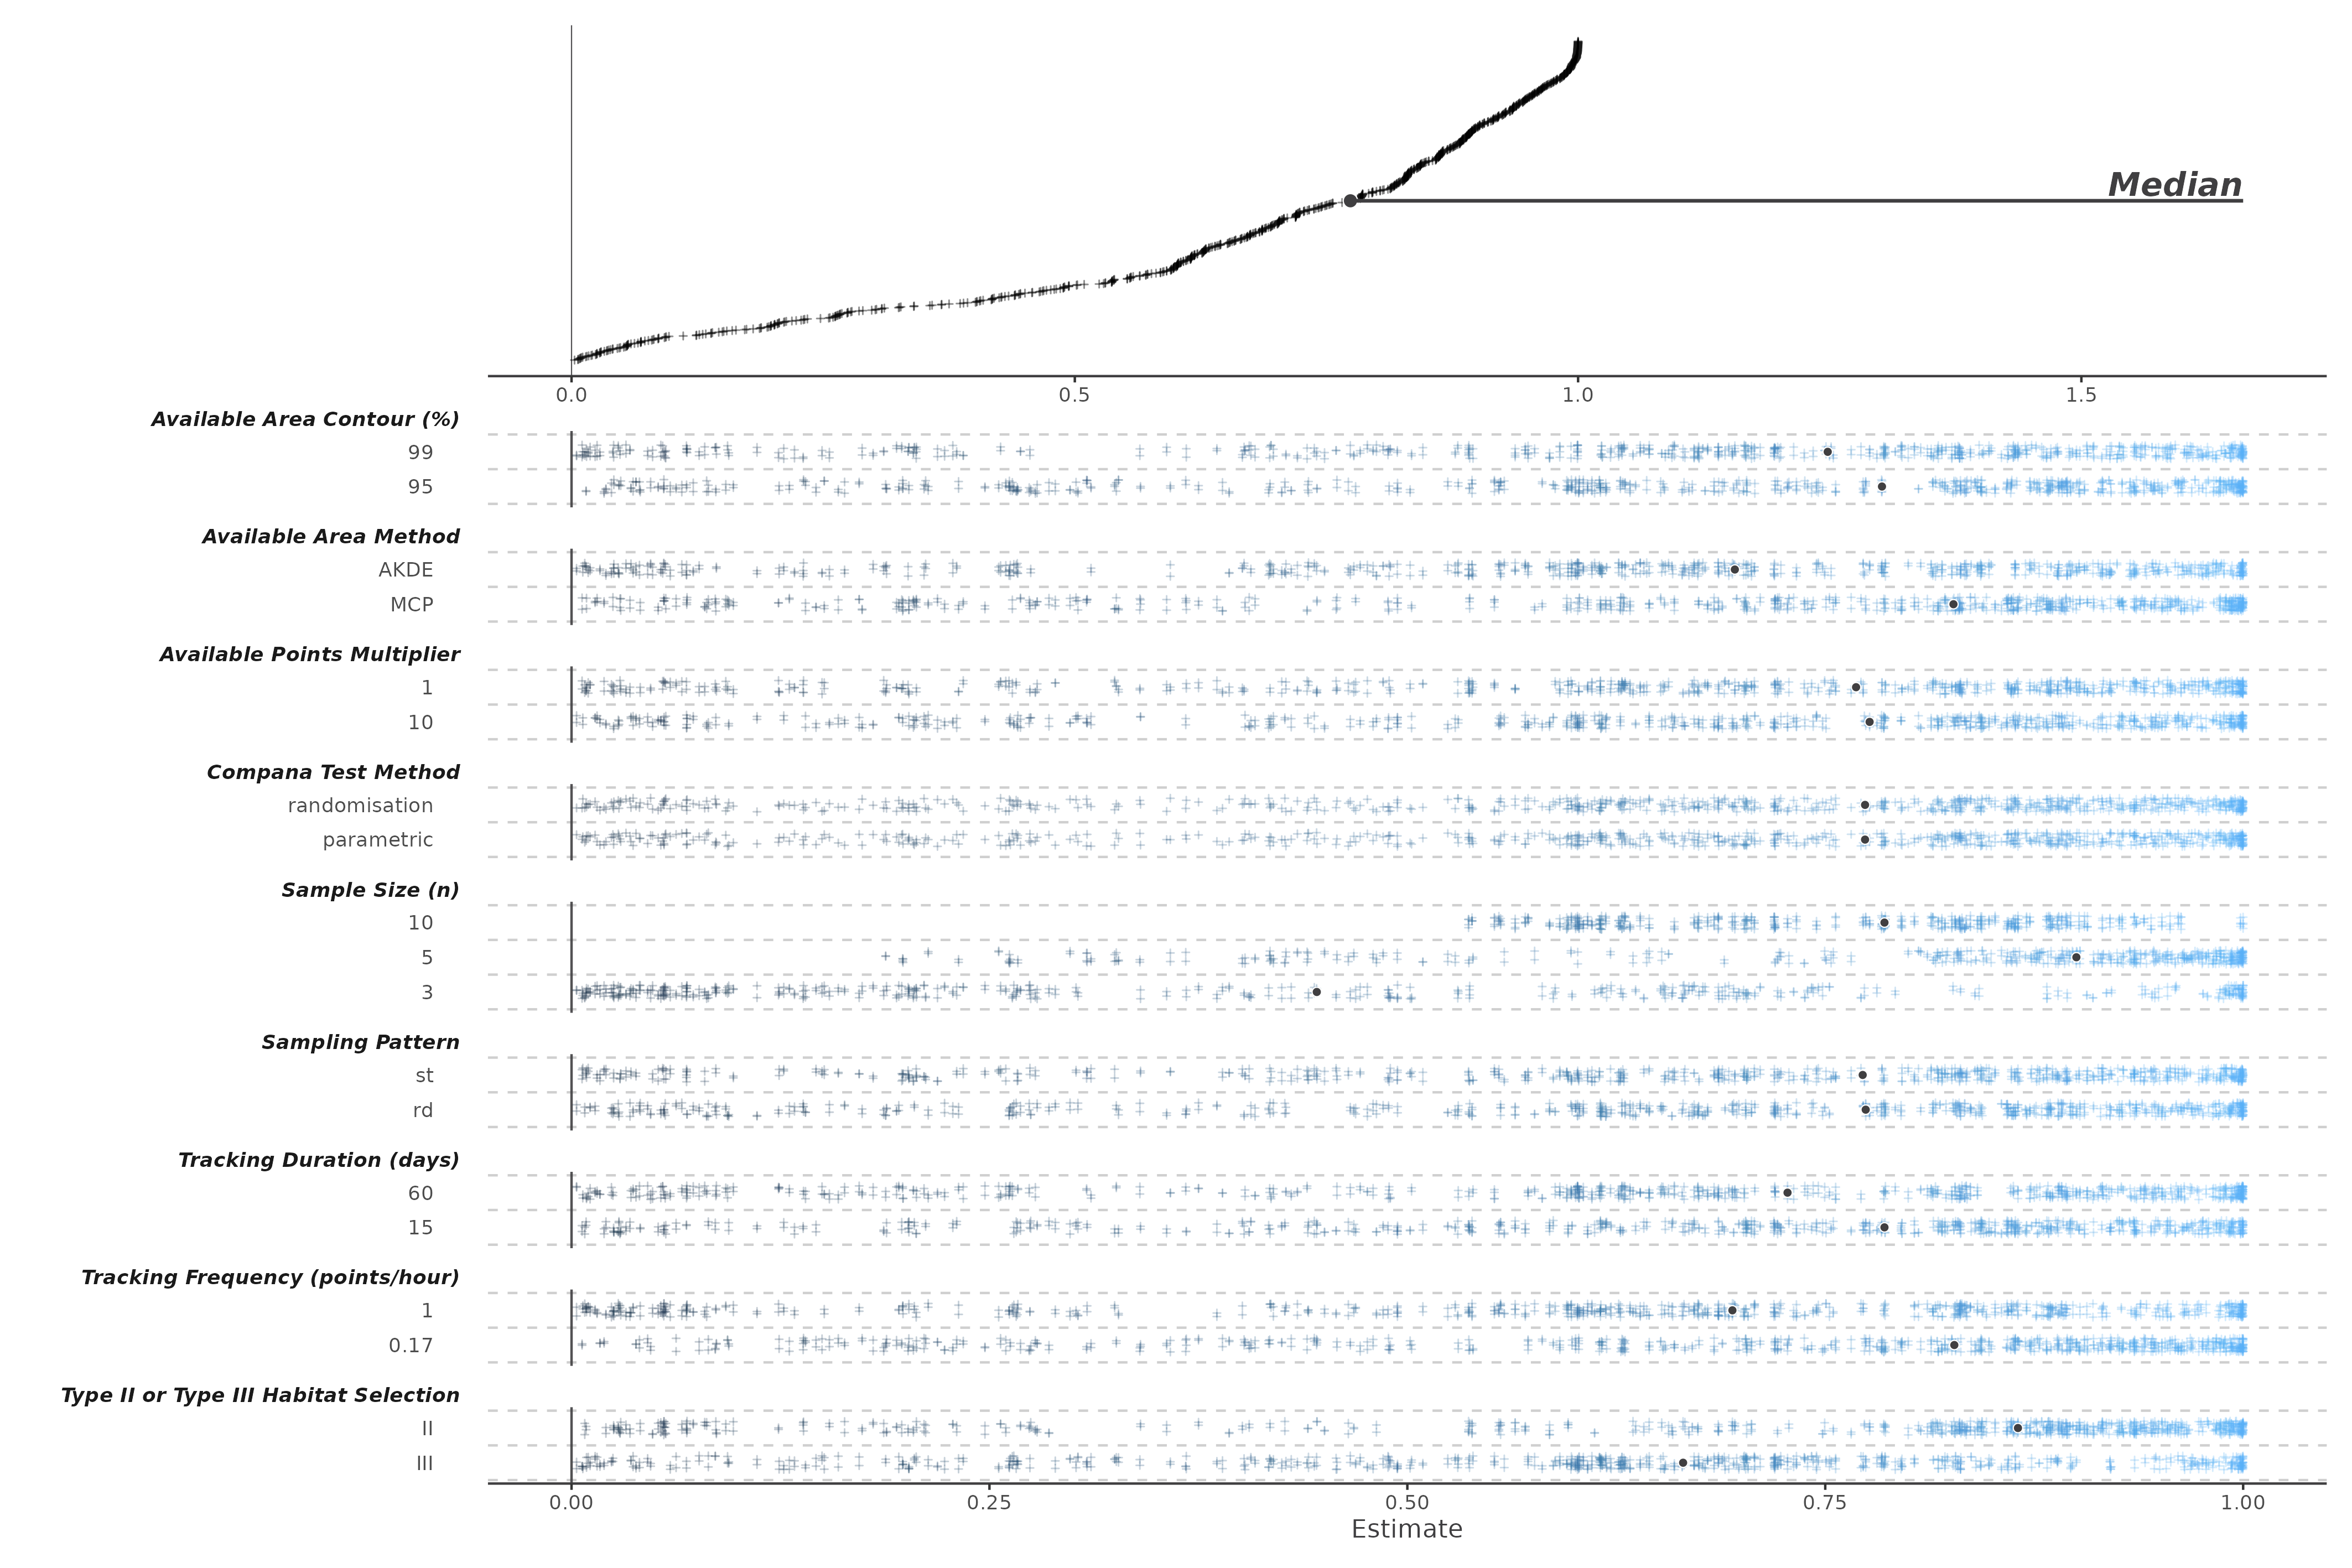
\includegraphics[width=1\linewidth]{../figures/area_specCurve} \caption{A specification curve showing habitat selection estimates resulting from the Compana (area-based) analysis pathways. Every point represents a separate estimate of habitat selection. The top plot shows all estimates organised by estimate strength. The lower plot shows the same estimates, but split by the analysis or sampling decisions. Solid circles are the medians for each choice.}\label{fig:specCurveArea}
\end{figure}

The specification curve generated from summarised Step Selection Functions (SSFs), similarly reveals a median estimate has agrees well with the simulated parametrisation for both selection and scrambled scenarios (Fig. \ref{fig:specCurveSSF}).
Also like the Compana curve, the SSF curve has far fewer results that indicate very low habitat preference in the positive selection scenario.
The majority of these lower estimates of habitat selection appear connected to the decision to use an non-integrated (standard) model formulation, and a decision to model averaging weighted by AIC.
The naively model averaged estimates are also much more tightly grouped with fewer estimates failing to correctly detect positive preference; the tighter grouping is also reflected in the scrambled selection scenario.

Outside the lower estimates, the clearest structure in the estimates results from different decisions in sample size and tracking regime.
The tracking regime decisions, frequency and duration, appear to shift the overall range of estimates but with limited impact on the variation.
By comparison, sample size increases appear to reduce the spread of estimates produced.

\begin{figure}
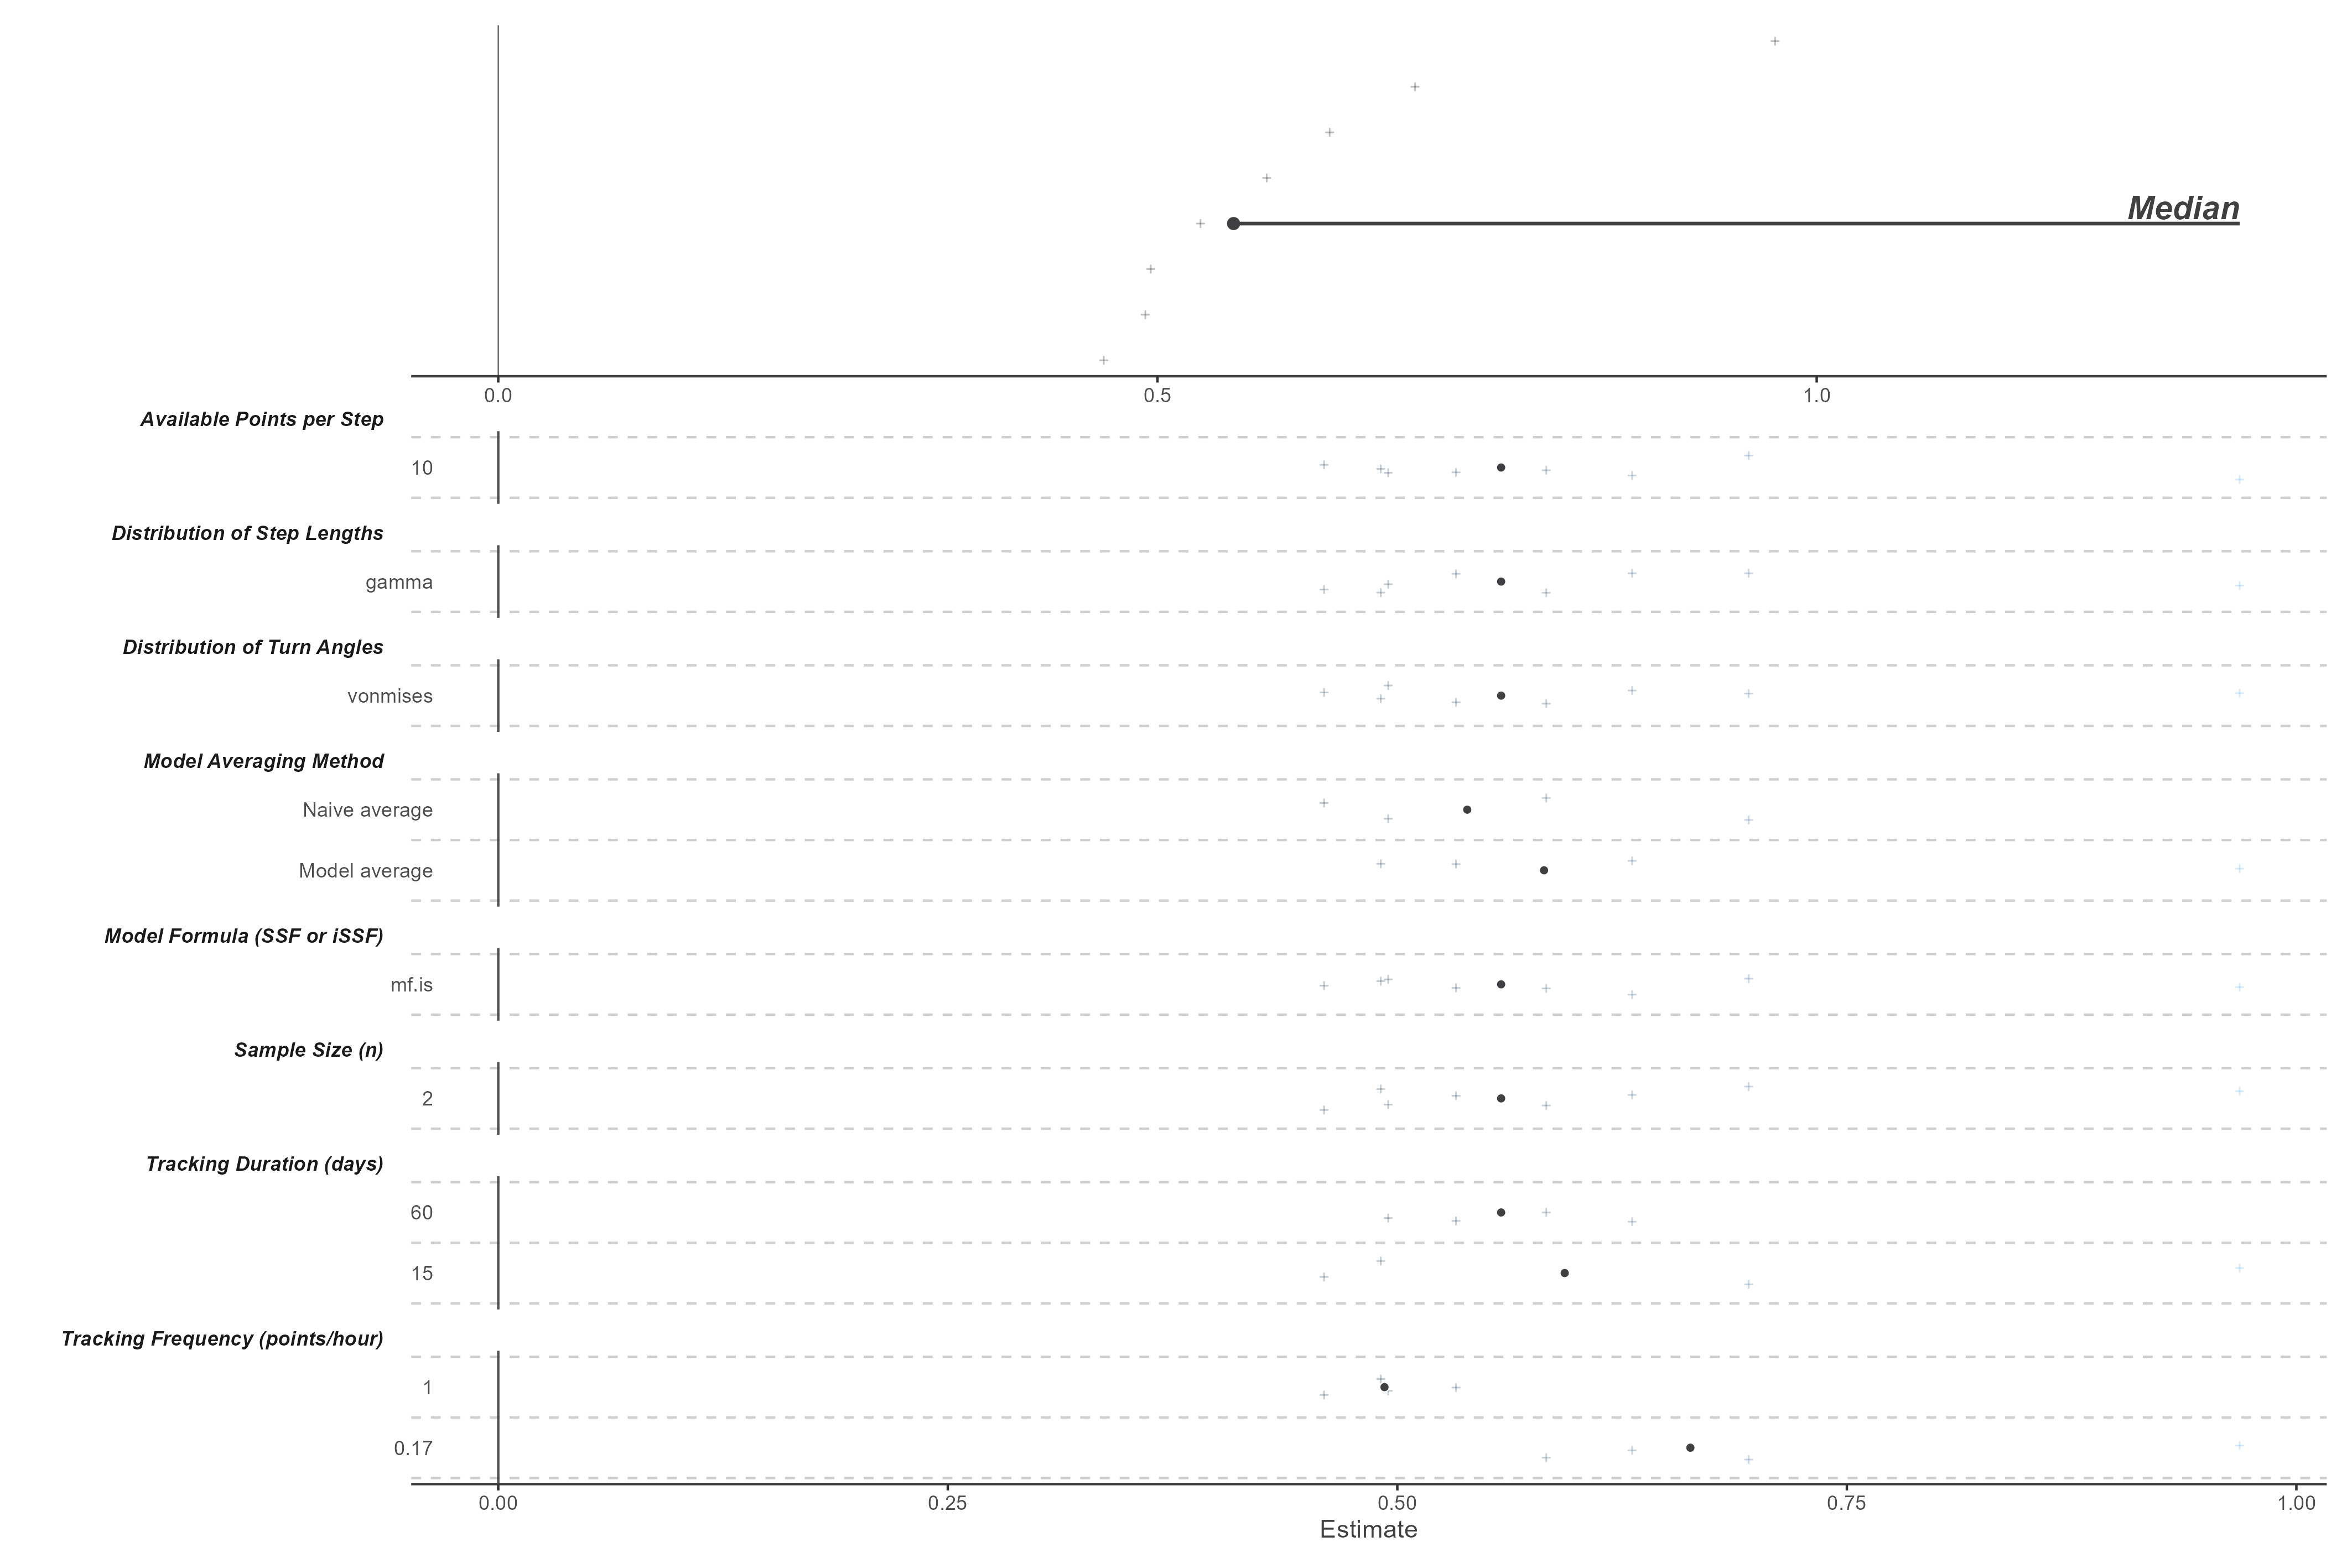
\includegraphics[width=1\linewidth]{../figures/ssf_specCurve} \caption{A specification curve showing habitat selection estimates resulting from the Step-selection Function (SSF) analysis pathways. Every point represents a separate estimate of habitat selection. The top plot shows all estimates organised by estimate strength. The lower plot shows the same estimates, but split by the analysis or sampling decisions. Solid circles are the medians for each choice.}\label{fig:specCurveSSF}
\end{figure}

The two-step model approach appears to have had the greatest difficultly consistently detecting the positive selection, but the median selection in the positive selection scenario is still greater than the median from the scrambled scenario (Fig. \ref{fig:specCurveTwoStep}).
Tracking frequency appears a critical decision in the two-step model with the 1 point per hour choice resulting in more detections of positive selection, and a tighter grouping of estimates.
The decision to integrate step and turn angle into the model formula appears similarly critical, with the choice not to include the step and turn angle results in in estimates more consistently positive in the positive selection scenario, and close to zero in the scrambled selection scenario.
The integrated model formulation appears to be largely responsible for the majrity of the variation in estimates.

\begin{figure}
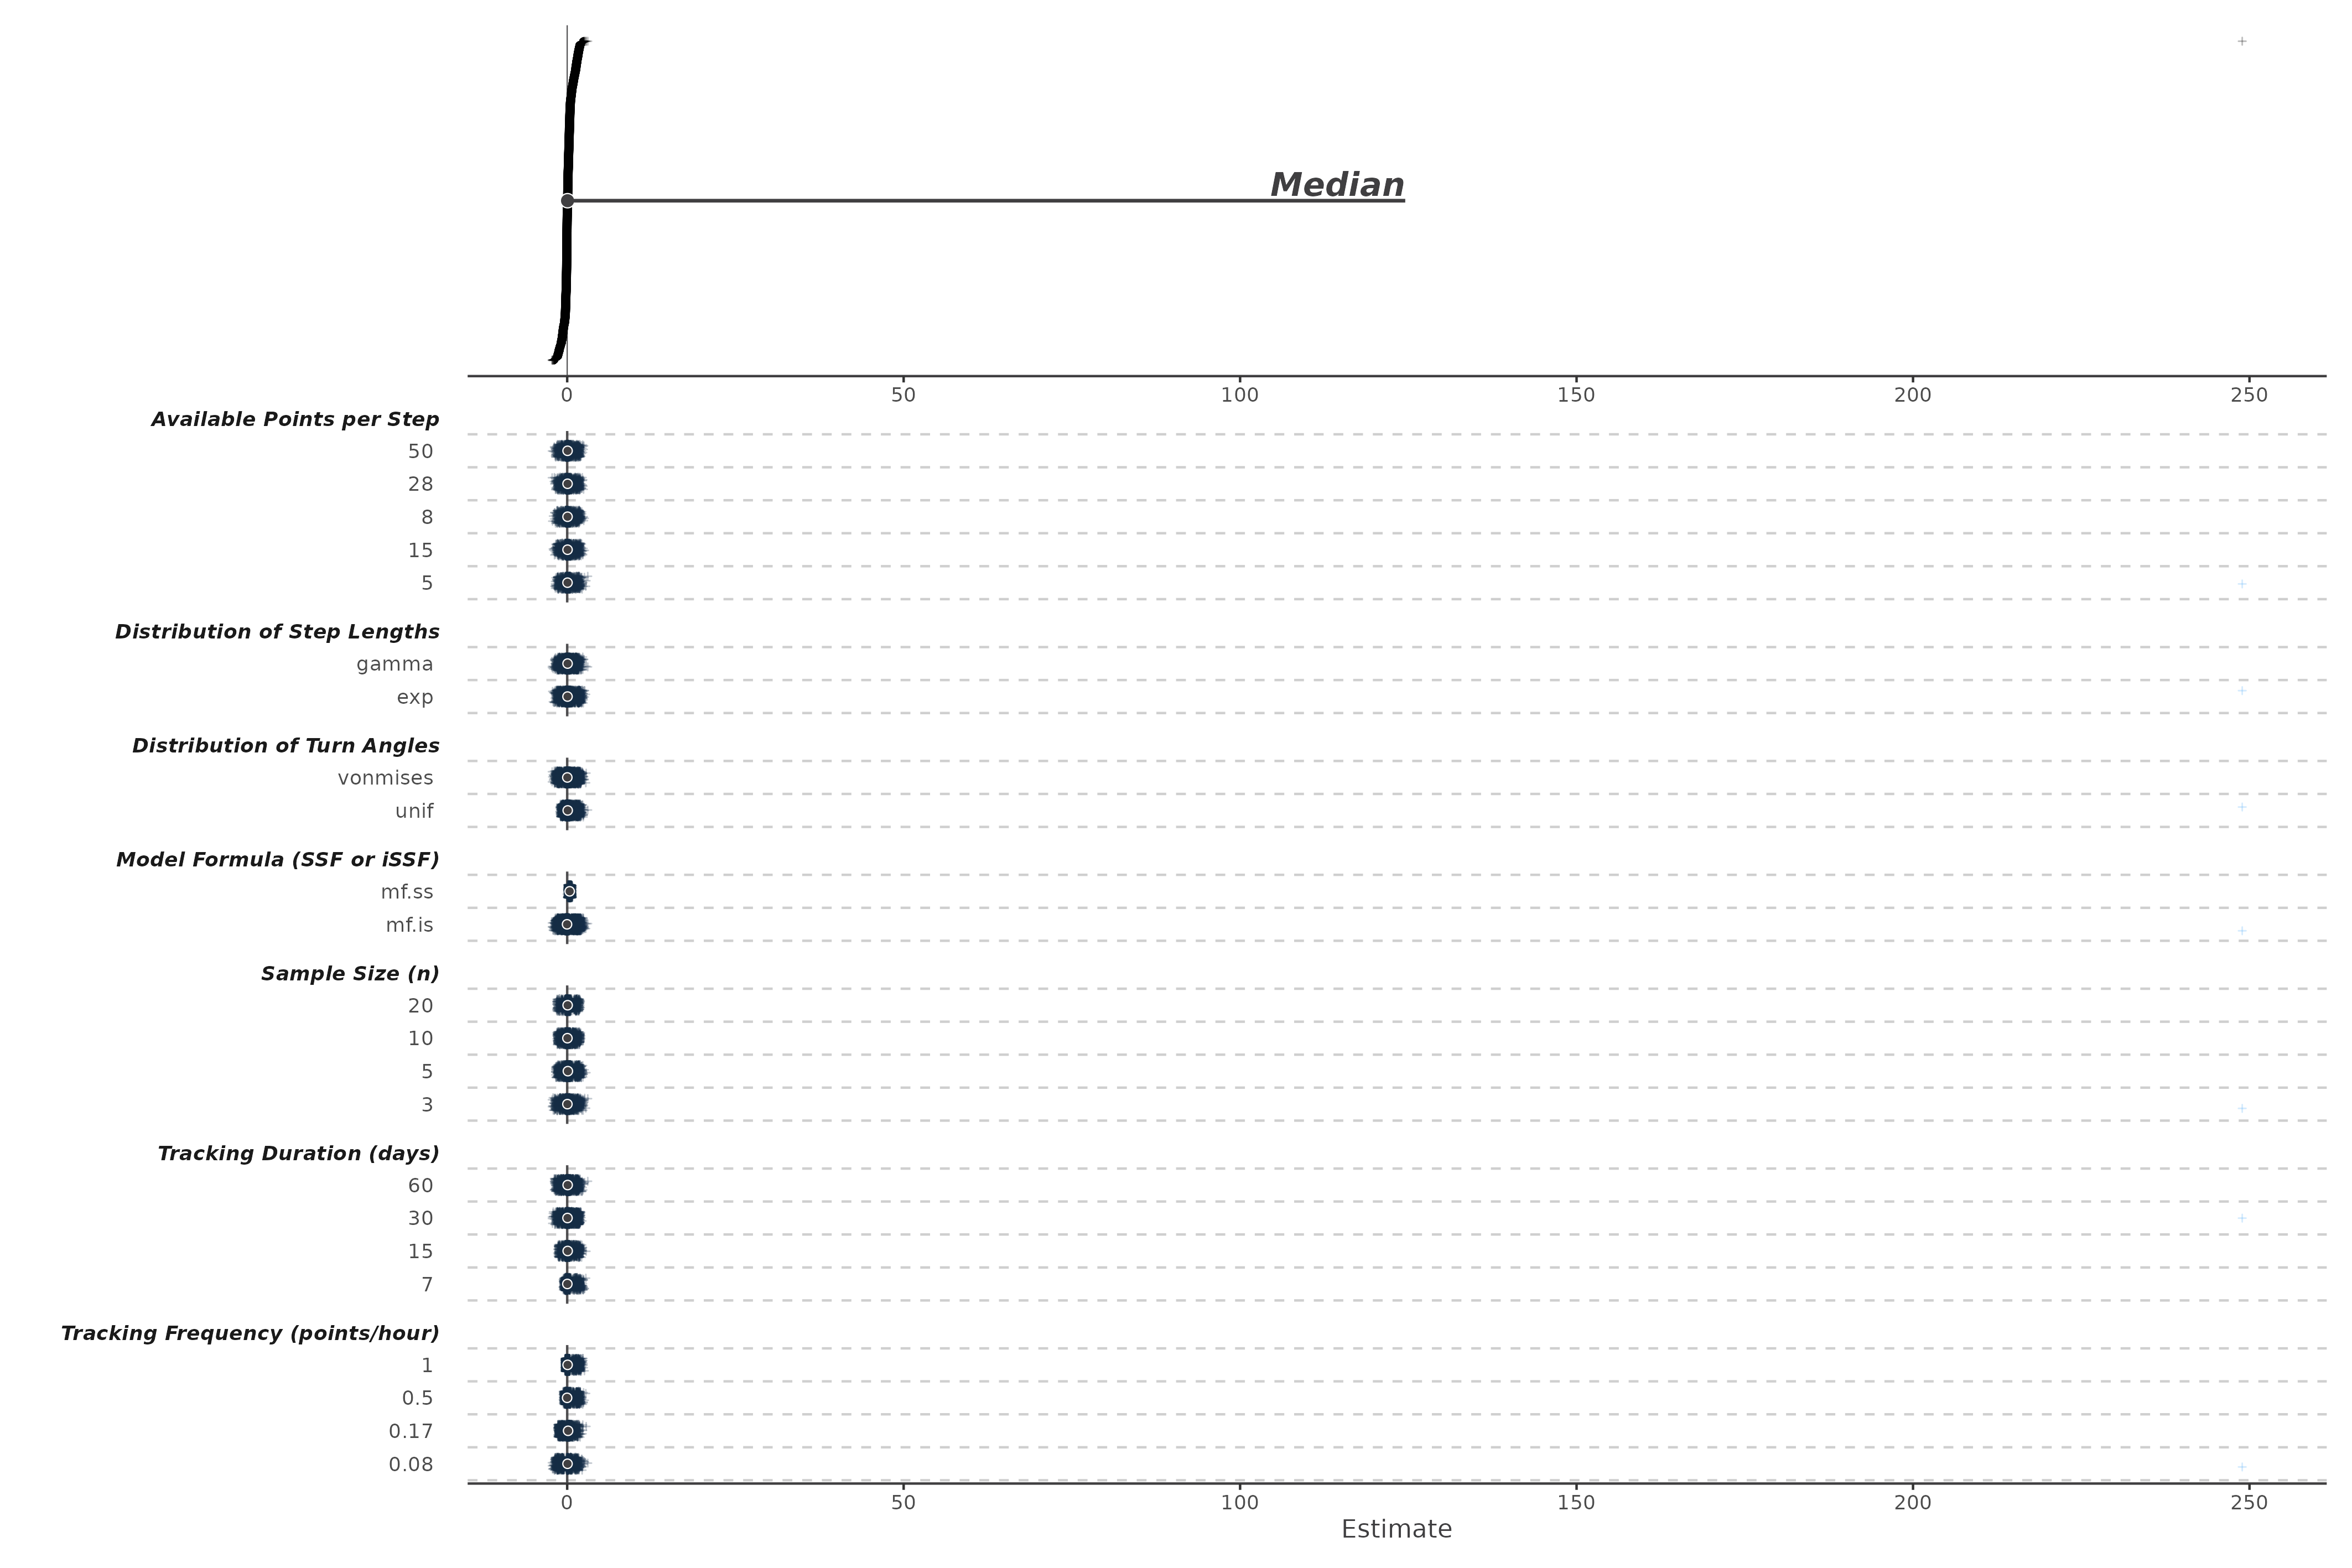
\includegraphics[width=1\linewidth]{../figures/twoStep_specCurve} \caption{A specification curve showing habitat selection estimates resulting from the Two-step analysis pathways. Every point represents a separate estimate of habitat selection. The top plot shows all estimates organised by estimate strength. The lower plot shows the same estimates, but split by the analysis or sampling decisions. Solid circles are the medians for each choice.}\label{fig:specCurveTwoStep}
\end{figure}

The Poisson based approach, like those before, shows that the vast majority of analysis pathways will result in the correct identification of positive preference for habitat 2 (Fig. \ref{fig:specCurvePois}), and centre on zero for the scrambled scenario.
Unlike the previous analyses the tracking duration did not have as clear an impact on the spread of estimates.
Sample size and tracking frequency did, with larger sample sizes and higher frequency leading to overall decreases in estimate spread.
Of particular note is that the majority of failures to detect positive preference occur when the sample size is three and at lower tracking frequencies.
The analysis decisions appear largely un-impactful, particularly the number of points per step.
Model formulation did have an impact, with the integrated formulation being more consistent at retrieving positive preference in the positive selection scenario, but the spread of estimates was much larger.
This spread increased associated with the integrated model formulation was similarly seen in the scrambled selection scenario, but resulted in near identical median estimates.

\begin{figure}
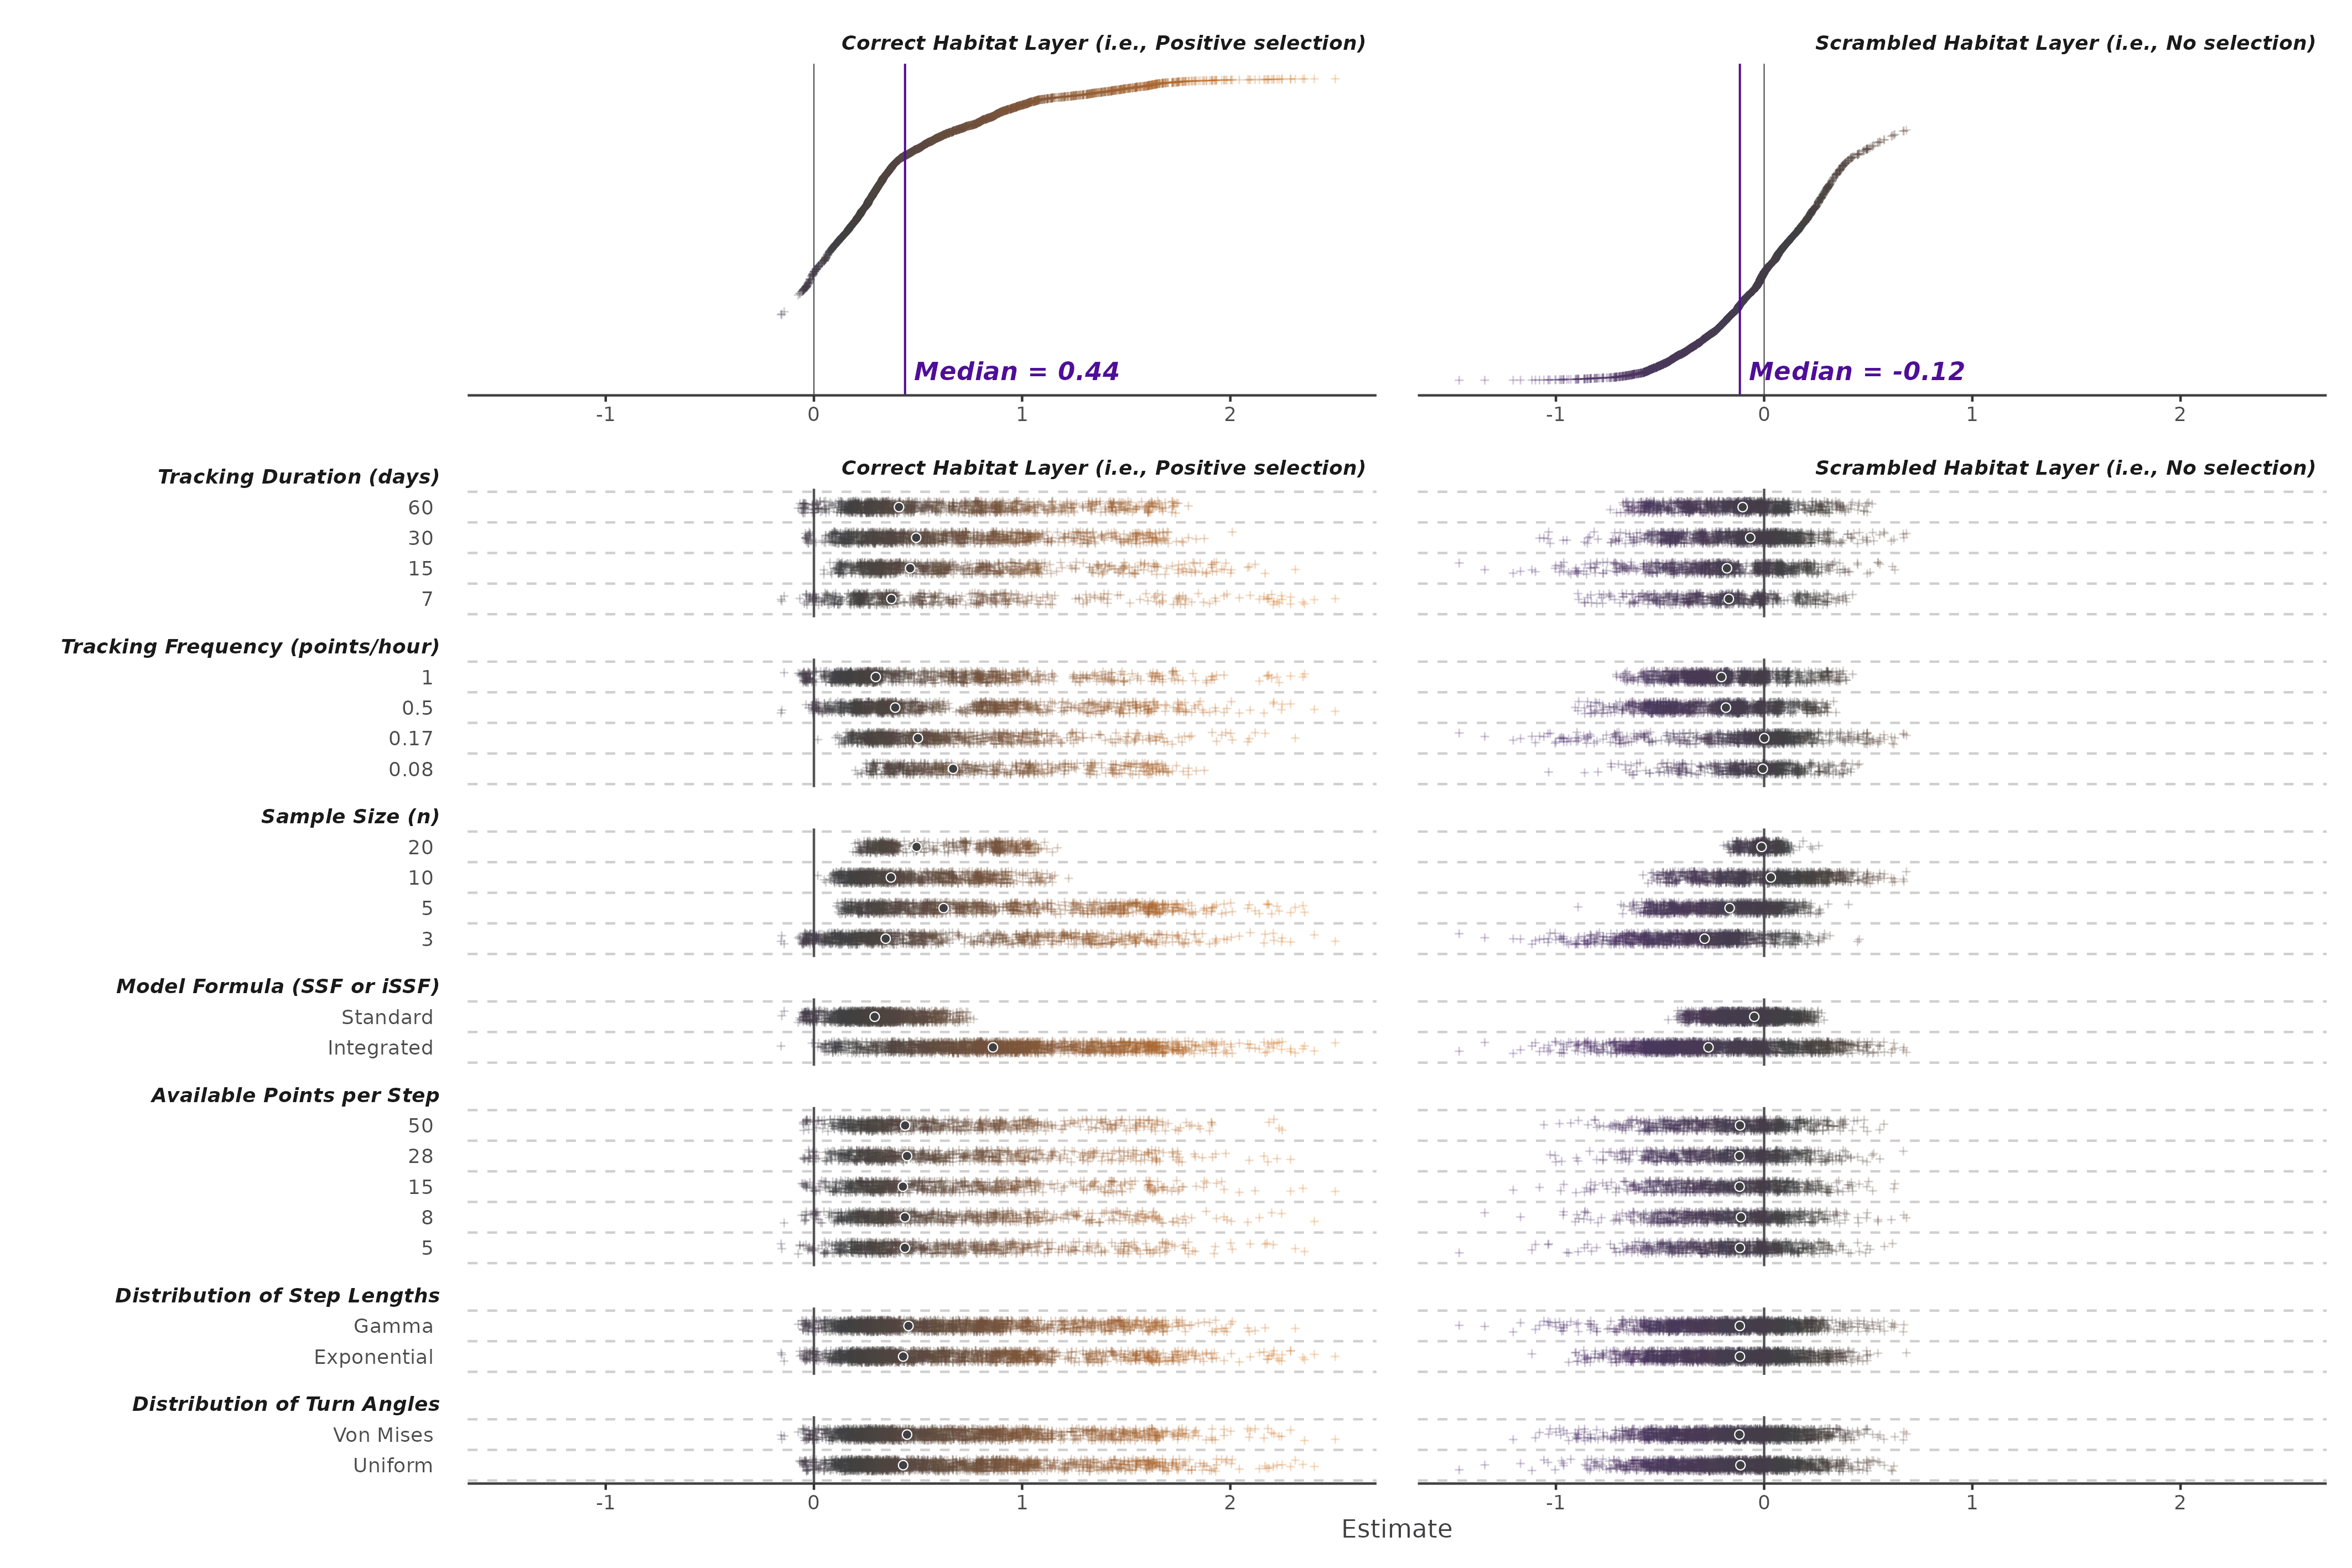
\includegraphics[width=1\linewidth]{../figures/pois_specCurve} \caption{A specification curve showing habitat selection estimates resulting from the Poisson analysis pathways. Every point represents a separate estimate of habitat selection. The top plot shows all estimates organised by estimate strength. The lower plot shows the same estimates, but split by the analysis or sampling decisions. Solid circles are the medians for each choice.}\label{fig:specCurvePois}
\end{figure}

\subsection{Model Results}\label{model-results}

We also used four Bayesian Regression Models to explore the impact of different decisions (Fig. \ref{fig:allEffectsPlot}), and whether those decisions can predict deviation from the median estimate (i.e., as a proxy for seeing which decisions lead to outlying extreme results).
The models provide a means to account for the variation that originates from stochasticity in the simulation and sampling; the shear number of final estimates can obscure patterns in specification curves.

The conditional \emph{R\textsuperscript{2}} values differed for the four models.
The Compana results model had a conditional \emph{R\textsuperscript{2}} of 0.32; whereas the SSF model returned 0.29; the Two-Step model returned 0.14; and the Poisson model returned 0.3.

The marginal \emph{R\textsuperscript{2}} represents the bulk of the conditional \emph{R\textsuperscript{2}} suggesting an important role for the fixed/population effects.
The Compana results model had a conditional \emph{R\textsuperscript{2}} of 0.18; whereas the SSF model returned 0.18; the Two-Step model returned 0.05; and the Poisson model returned 0.11

The area-based Compana approach seemed more insensitive to sample size than the other methods (\(\beta\) 0.28; 95\% HDCI 0.10 - 0.47), instead benefiting from increases in tracking duration (\(\beta\) 0.06; 95\% HDCI 0.04 - 0.07) and frequency (\(\beta\) 0.12; 95\% HDCI 0.10 - 0.13; Fig. \ref{fig:effectPlotArea}).
This contrasts strongly with the Poisson model approach, where all increases in sampling intensity lead to marked reductions in deviation from the median estimate: sample size (\(\beta\) -0.02; 95\% HDCI -0.06 - 0.02), tracking duration (\(\beta\) -0.02; 95\% HDCI -0.02 - -0.01), and tracking frequency (\(\beta\) -0.02; 95\% HDCI -0.03 - -0.02; Fig. \ref{fig:effectPlotPois}).
The other two methods fall in-between with the sampling having a smaller impact.
The Step Selection model approach still benefited from increasing sampling duration (\(\beta\) -0.04; 95\% HDCI -0.04 - -0.04) and frequency, but the impact on increasing sample size was not apparent (\(\beta\) -0.04; 95\% HDCI -0.04 - -0.04; Fig. \ref{fig:effectPlotSSF}).

The points per step decision holds the largest improvement in terms of deviation from the median; the Poisson model approach was aided greatly by increases to the number of random points per step (\(\beta\) 0.00; 95\% HDCI 0.00 - 0.01).
This clear effect highlights the limitations of relying solely on the specification curves, where this pattern was not clearly visible.
Unlike the points per step decision the naive averaging of the step selection models leading to a smaller spread of estimates is visible in the specification curve and confirmed by model beta estimate (\(\beta\) -0.18; 95\% HDCI -0.18 - -0.17).

The most mixed decision is the use of model formulation that includes the step and turn angles (i.e., integrated versus not integrated).
Here we see the benefits of including the step and turn angles in the model formula for the summarised SSF approach (\(\beta\) 0.04; 95\% HDCI 0.04 - 0.05), but a contrasting effect for both the Two-step (\(\beta\) -0.17; 95\% HDCI -0.17 - -0.16) and Poisson approaches (\(\beta\) -0.37; 95\% HDCI -0.38 - -0.36) where the not integrated formula tends to reduce the spread of estimates (Fig. \ref{fig:effectPlotSSF}.

The area based approach had a number of unique decisions.
Largely the decisions associated with defining the available area had a large impact that those linked to generating the random points (Fig. \ref{fig:effectPlotArea}).
In brief, the use of MCPs (\(\beta\) -0.16; 95\% HDCI -0.19 - -0.13), larger contours (areas) (\(\beta\) 0.05; 95\% HDCI 0.03 - 0.06), and type III designs (\(\beta\) -0.29; 95\% HDCI -0.32 - -0.26) tended to lead to more variable results.
The use of larger contours and type III designs appear to contradict each other, as one would tend towards a larger area, whereas the latter would be a more limited area based.

\begin{figure}
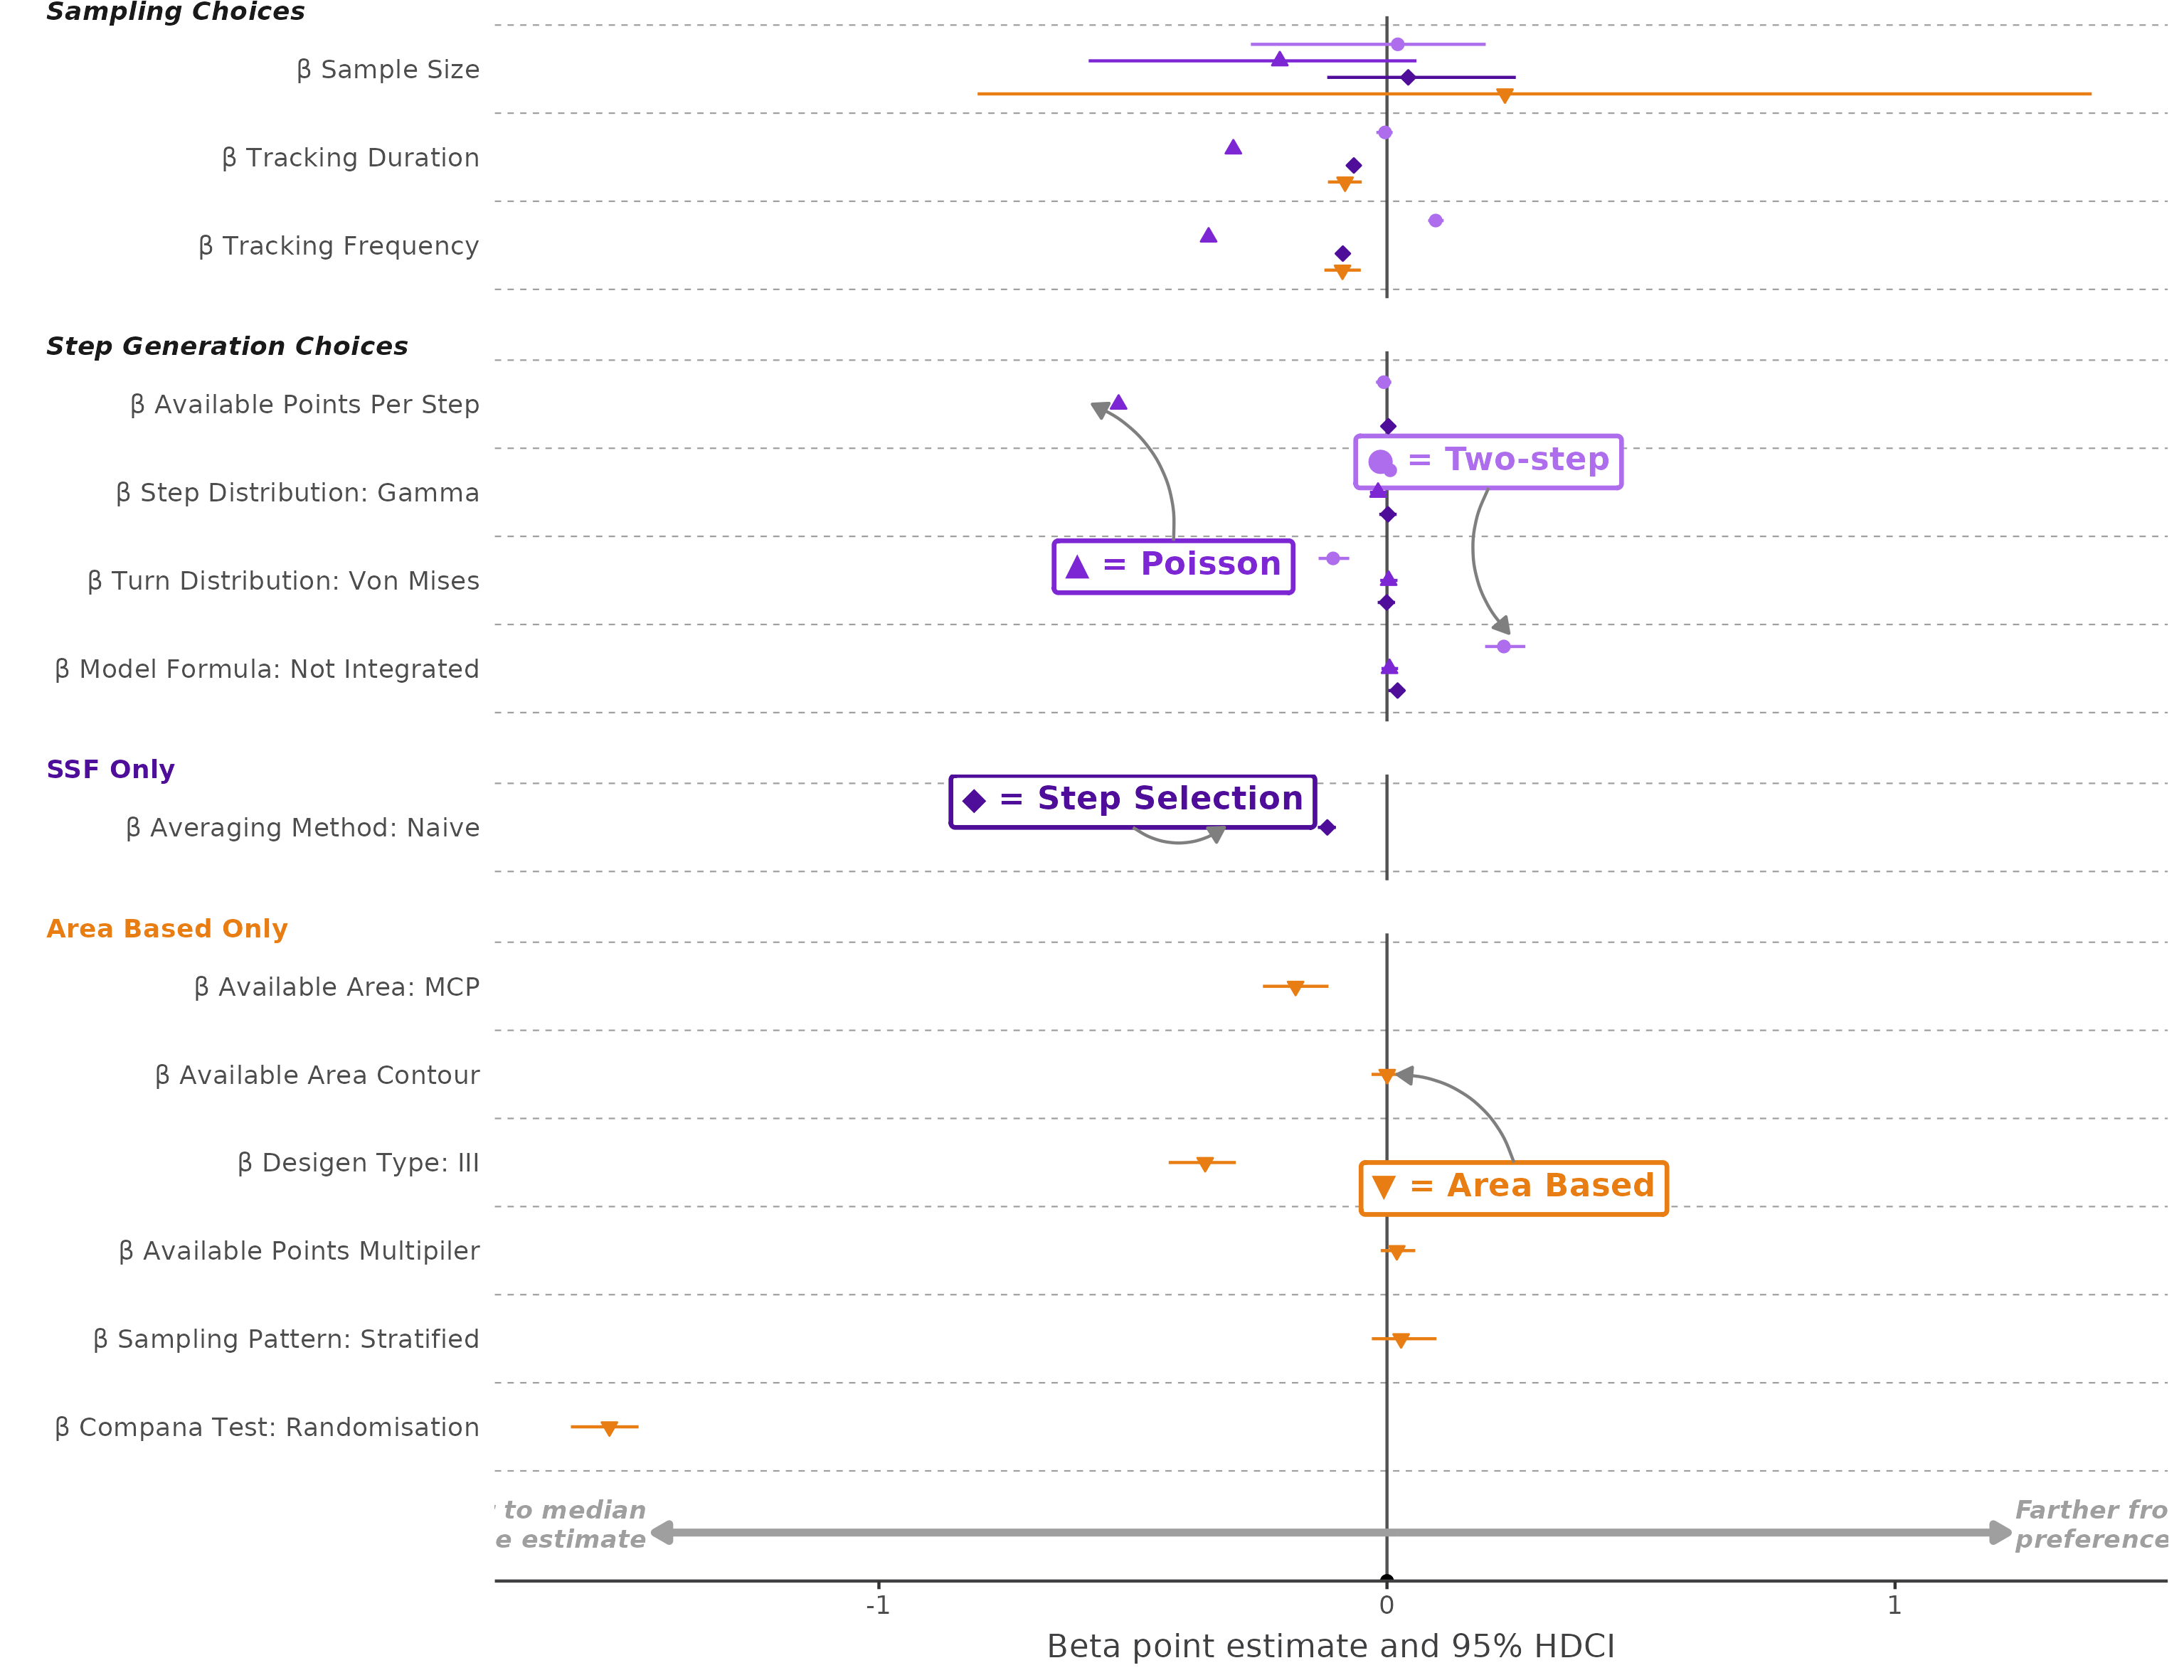
\includegraphics[width=1\linewidth]{../figures/_allEffectsPlot} \caption{Beta coefs}\label{fig:allEffectsPlot}
\end{figure}

\section{Discussion}\label{discussion}

The multiverse approach highlights the diverse array of answers one can obtain even when analysing the same data, simulated using the same parameters.
Fortunately the vast majority of the answers from the analysis end points agree, and correctly recover the positive habitat selection programmed into the simulated animals.
This broad agreement is cause of optimism, suggesting that the potentially deviating analysis choices made my researchers largely converge to an agreement --albeit within this given simulated scenario and given habitat preference strength.

Very much mirroring previous multiverse efforts, the largest effect on whether an estimate was close to the median estimate came from decisions concerning sampling.
The summarised Step Selection (SSF) approach as well as the Poisson model benefited the most from increasing the data quantity.

\subsection{Multiverse in context}\label{multiverse-in-context}

While the multiverse can help us explore the possible answers that can come from a given dataset, they cannot provide guidance on which of those answers is correct.
The creation of the multiverse is subject to the same decision making procedure that any single given pathway is: what decisions to include, how to vary the choices.
Therefore, the overall median or mean answer is heavily dependent on the construction of the multiverse.
Additionally, the choices and resulting analysis pathways are not equally as valid, nor equally likely to be undertaken by a researcher.
This means the multiverse of answers may provide some insight on spread of estimates, but should not be directly interpreted as providing more or less support for a given estimate based on the distribution of estimates.
We can take this issue further, reminding ourselves that agreement is not necessarily a reliable proxy for accuracy (\citeproc{ref-devezer_case_2021}{Devezer et al., 2021}).
A better model reflecting the mechanistic reality of the study system is preferable to a suite of models that agree but converge on a less accurate answer.
An example in the conducted multiverse: we used AKDEs and MCPs as two alternative definitions of availability for the area based method.
Arguably we should have excluded the MCP choice in favour of the AKDE choice, as the latter does a better job at capturing the movement processes/patterns underlying animal space-use.
Despite this the frequency of MCP use in spatial ecology (\citeproc{ref-crane_lots_2021}{Crane et al., 2021}), we felt, warranted its inclusion as a conceivable choice.
Judgement calls such as this are unavoidable, and determining whether a model better reflects the underlying system can be exceptionally difficult outside of simulated ``known-truth'' scenarios.

When we are uncertain of the mechanism, or unable to truly model the vast complexity of the system (very frequent in ecology), then informed agreement may be our best option.
Recent efforts looking at how many researchers answer the same question from the same dataset reveals that these judgement calls result in different answers (\citeproc{ref-gould_same_2023}{Gould et al., 2023}).
In many ways the more organic real-world results from Gould et al. (\citeproc{ref-gould_same_2023}{2023}) reflect the multiverse results presented here --a general agreement on direction, but variation in uncertainty and magnitude.
What differs, is that here we know the simulated correct answer is a positive effect, in Gould et al. (\citeproc{ref-gould_same_2023}{2023}) the truth is unknown and so we rely on the good agreement of many independent informed analyses.
The logistics of organising researchers to assess uncertainty in analyses is infeasible on a broader scale.
The multiverse approach presents a complementary method for assessing the scope of research choice on final results --albeit more vulnerable to the individual researcher's biases and potentially limited to analyses with lower computational costs.

We have avoided suggesting rules or guides based on these results, instead suggesting broad trends.
The diverse array of species tracked and the habitat's which they reside makes specific guidance nigh impossible without informed assumptions tailored to a given study system.
We simulated a nocturnal badger-like animal for this exploration.
This simualted badger occupied a number of shelter sites and routinely returned to them.
A routine use of shelter site in a the preferred habitat would mean that missing those sites/locations is unlikely with a reasonably frequent tracking regime.
Alternatively, one can imagine an animal with more limited site fidelity, where the use of preferred habitat is more fleeting or temporally inconsistent.
In this instance one may find a reduction in tracking frequency to dramatically alter the estimates retrieved.
Previous work with SSF has already highlighted the importance of more random locations per step for identifying use of smaller/rarer habitat types (\citeproc{ref-thurfjell_applications_2014}{Thurfjell, Ciuti \& Boyce, 2014}).
Some methods, such as Resource Selection Functions, have the means of estimating the required data quantity to detect a given strength of selection in a given landscape, and provide a guide to how consistent results would be from that dataset (\citeproc{ref-street_solving_2021}{Street et al., 2021}).
These methods still require informed decisions to be made concerning the strength of selection that is of interest as well as how to define the landscape, but complement the goal of the multiverse assessment with a more rigorously mathematical approach.

\subsection{Conclusions}\label{conclusions}

We would the following questions be asked concerning the outputs of a multiverse: how much variation in estimates is cause for concern? Are there estimates that would alter the final conclusions?

\section{Acknowledgements}\label{acknowledgements}

This work was supported by the Natural Environment Research Council (NERC) via the IAPETUS2 Doctoral Training Partnership held by Benjamin Michael Marshall (grant reference NE/S007431/1).

\section{Software availablity}\label{software-availablity}

In addition to packages already mentioned in the methods we also used the following.

We used \emph{R} v.4.2.2 (\citeproc{ref-base}{R Core Team, 2023}) via \emph{RStudio} v.2023.09.1 (\citeproc{ref-rstudio}{RStudio Team, 2022}).
We used \emph{here} v.1.0.1 (\citeproc{ref-here}{Müller, 2020}) and \emph{qs} v.0.26.3 (\citeproc{ref-qs}{Ching, 2023}) to manage directory addresses and saved objects.

We used \emph{raster} v.3.6.26 (\citeproc{ref-raster}{Hijmans, 2023}) and \emph{RandomFields} v.3.3.14 (\citeproc{ref-RandomFields}{Schlather et al., 2015}) to aid landscape raster creation alongside NLMR v.1.1.1 (\citeproc{ref-NLMR}{Sciaini et al., 2018}).

We used \emph{ggplot2} v.3.5.1 for creating figures (\citeproc{ref-ggplot2}{Wickham, 2016}), with the expansions: \emph{patchwork} v.1.2.0 (\citeproc{ref-patchwork}{Pedersen, 2022}), \emph{ggridges} v.0.5.6 (\citeproc{ref-ggridges}{Wilke, 2022}), \emph{ggdist} v.3.3.2 (\citeproc{ref-ggdist}{Kay, 2023a}), and \emph{ggtext} v.0.1.2 (\citeproc{ref-ggtext}{Wilke \& Wiernik, 2022}).

We used \emph{brms} v.2.21.0 (\citeproc{ref-brms}{Bürkner, 2021}) to run Bayesian models, with diagnostics generated used \emph{bayesplot} v.1.11.1 (\citeproc{ref-bayesplot}{Gabry et al., 2019}), \emph{tidybayes} v.3.0.6 (\citeproc{ref-tidybayes}{Kay, 2023b}), and \emph{performance} v.0.11.0 (\citeproc{ref-performance}{Lüdecke et al., 2021}).

We used the \emph{dplyr} v.1.1.4 (\citeproc{ref-dplyr}{Wickham et al., 2023}), \emph{tibble} v.3.2.1 (\citeproc{ref-tibble}{Müller \& Wickham, 2023}),
and \emph{stringr} v.1.5.1 (\citeproc{ref-stringr}{Wickham, 2022}) packages for data manipulation.

We used \emph{sp} v.2.1.4 (\citeproc{ref-sp}{Bivand, Pebesma \& Gomez-Rubio, 2013}), \emph{move} v.4.2.4 (\citeproc{ref-move}{Kranstauber, Smolla \& Scharf, 2023}) for manipulation of spatial data and estimation of space use not otherwise mentioned in the methods.

We used rmarkdown v.2.27 (\citeproc{ref-rmarkdown2018}{Xie, Allaire \& Grolemund, 2018}; \citeproc{ref-rmarkdown2020}{Xie, Dervieux \& Riederer, 2020}; \citeproc{ref-rmarkdown2023}{Allaire et al., 2023}), bookdown v.0.39 (\citeproc{ref-bookdown2016}{Xie, 2016}, \citeproc{ref-R-bookdown}{2022}), tinytex v.0.51 (\citeproc{ref-tinytex2019}{Xie, 2019}, \citeproc{ref-tinytex2023}{2023a}), and knitr v.1.47 (\citeproc{ref-knitr2014}{Xie, 2014}, \citeproc{ref-knitr2015}{2015}, \citeproc{ref-knitr2023}{2023b}) packages to generate type-set outputs.

We generated R package citations with the aid of \emph{grateful} v.0.2.4 (\citeproc{ref-grateful}{Francisco Rodríguez-Sánchez, Connor P. Jackson \& Shaurita D. Hutchins, 2023}).

\section{Data availabilty}\label{data-availabilty}

\clearpage

\section{Supplementary Material}\label{supplementary-material}

\begin{figure}
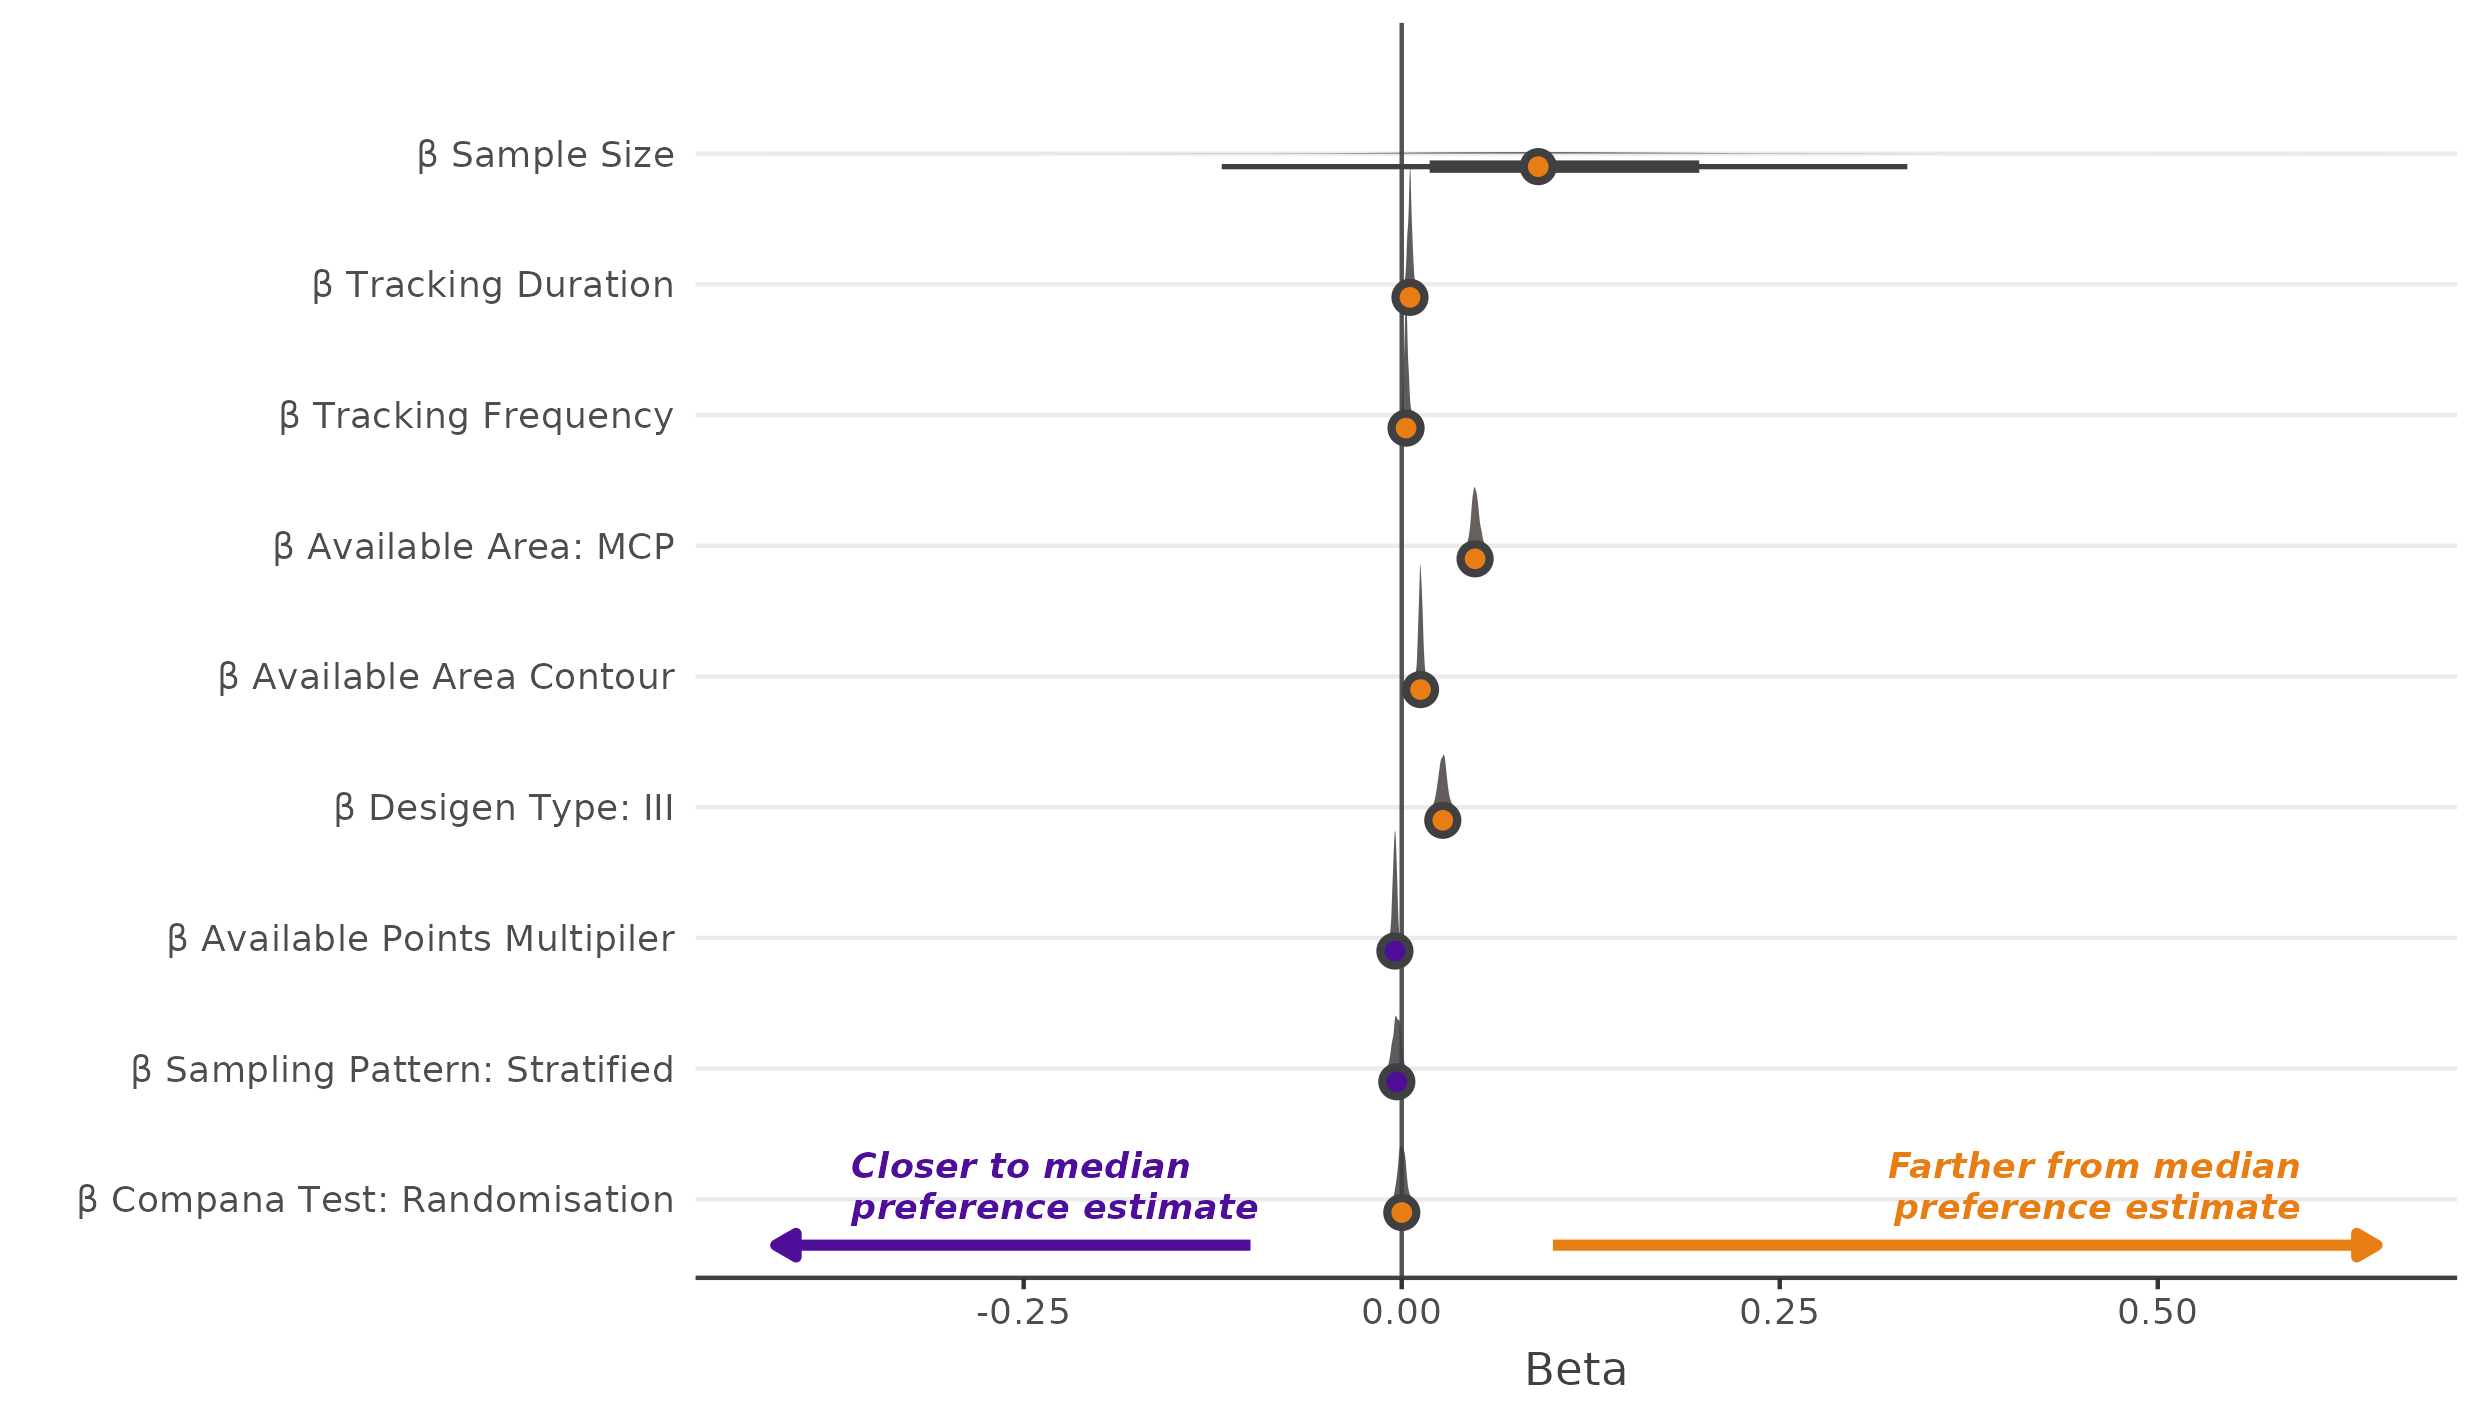
\includegraphics[width=1\linewidth]{../figures/areaBrms_effectsPlot} \caption{Beta coefs}\label{fig:effectPlotArea}
\end{figure}

\begin{figure}
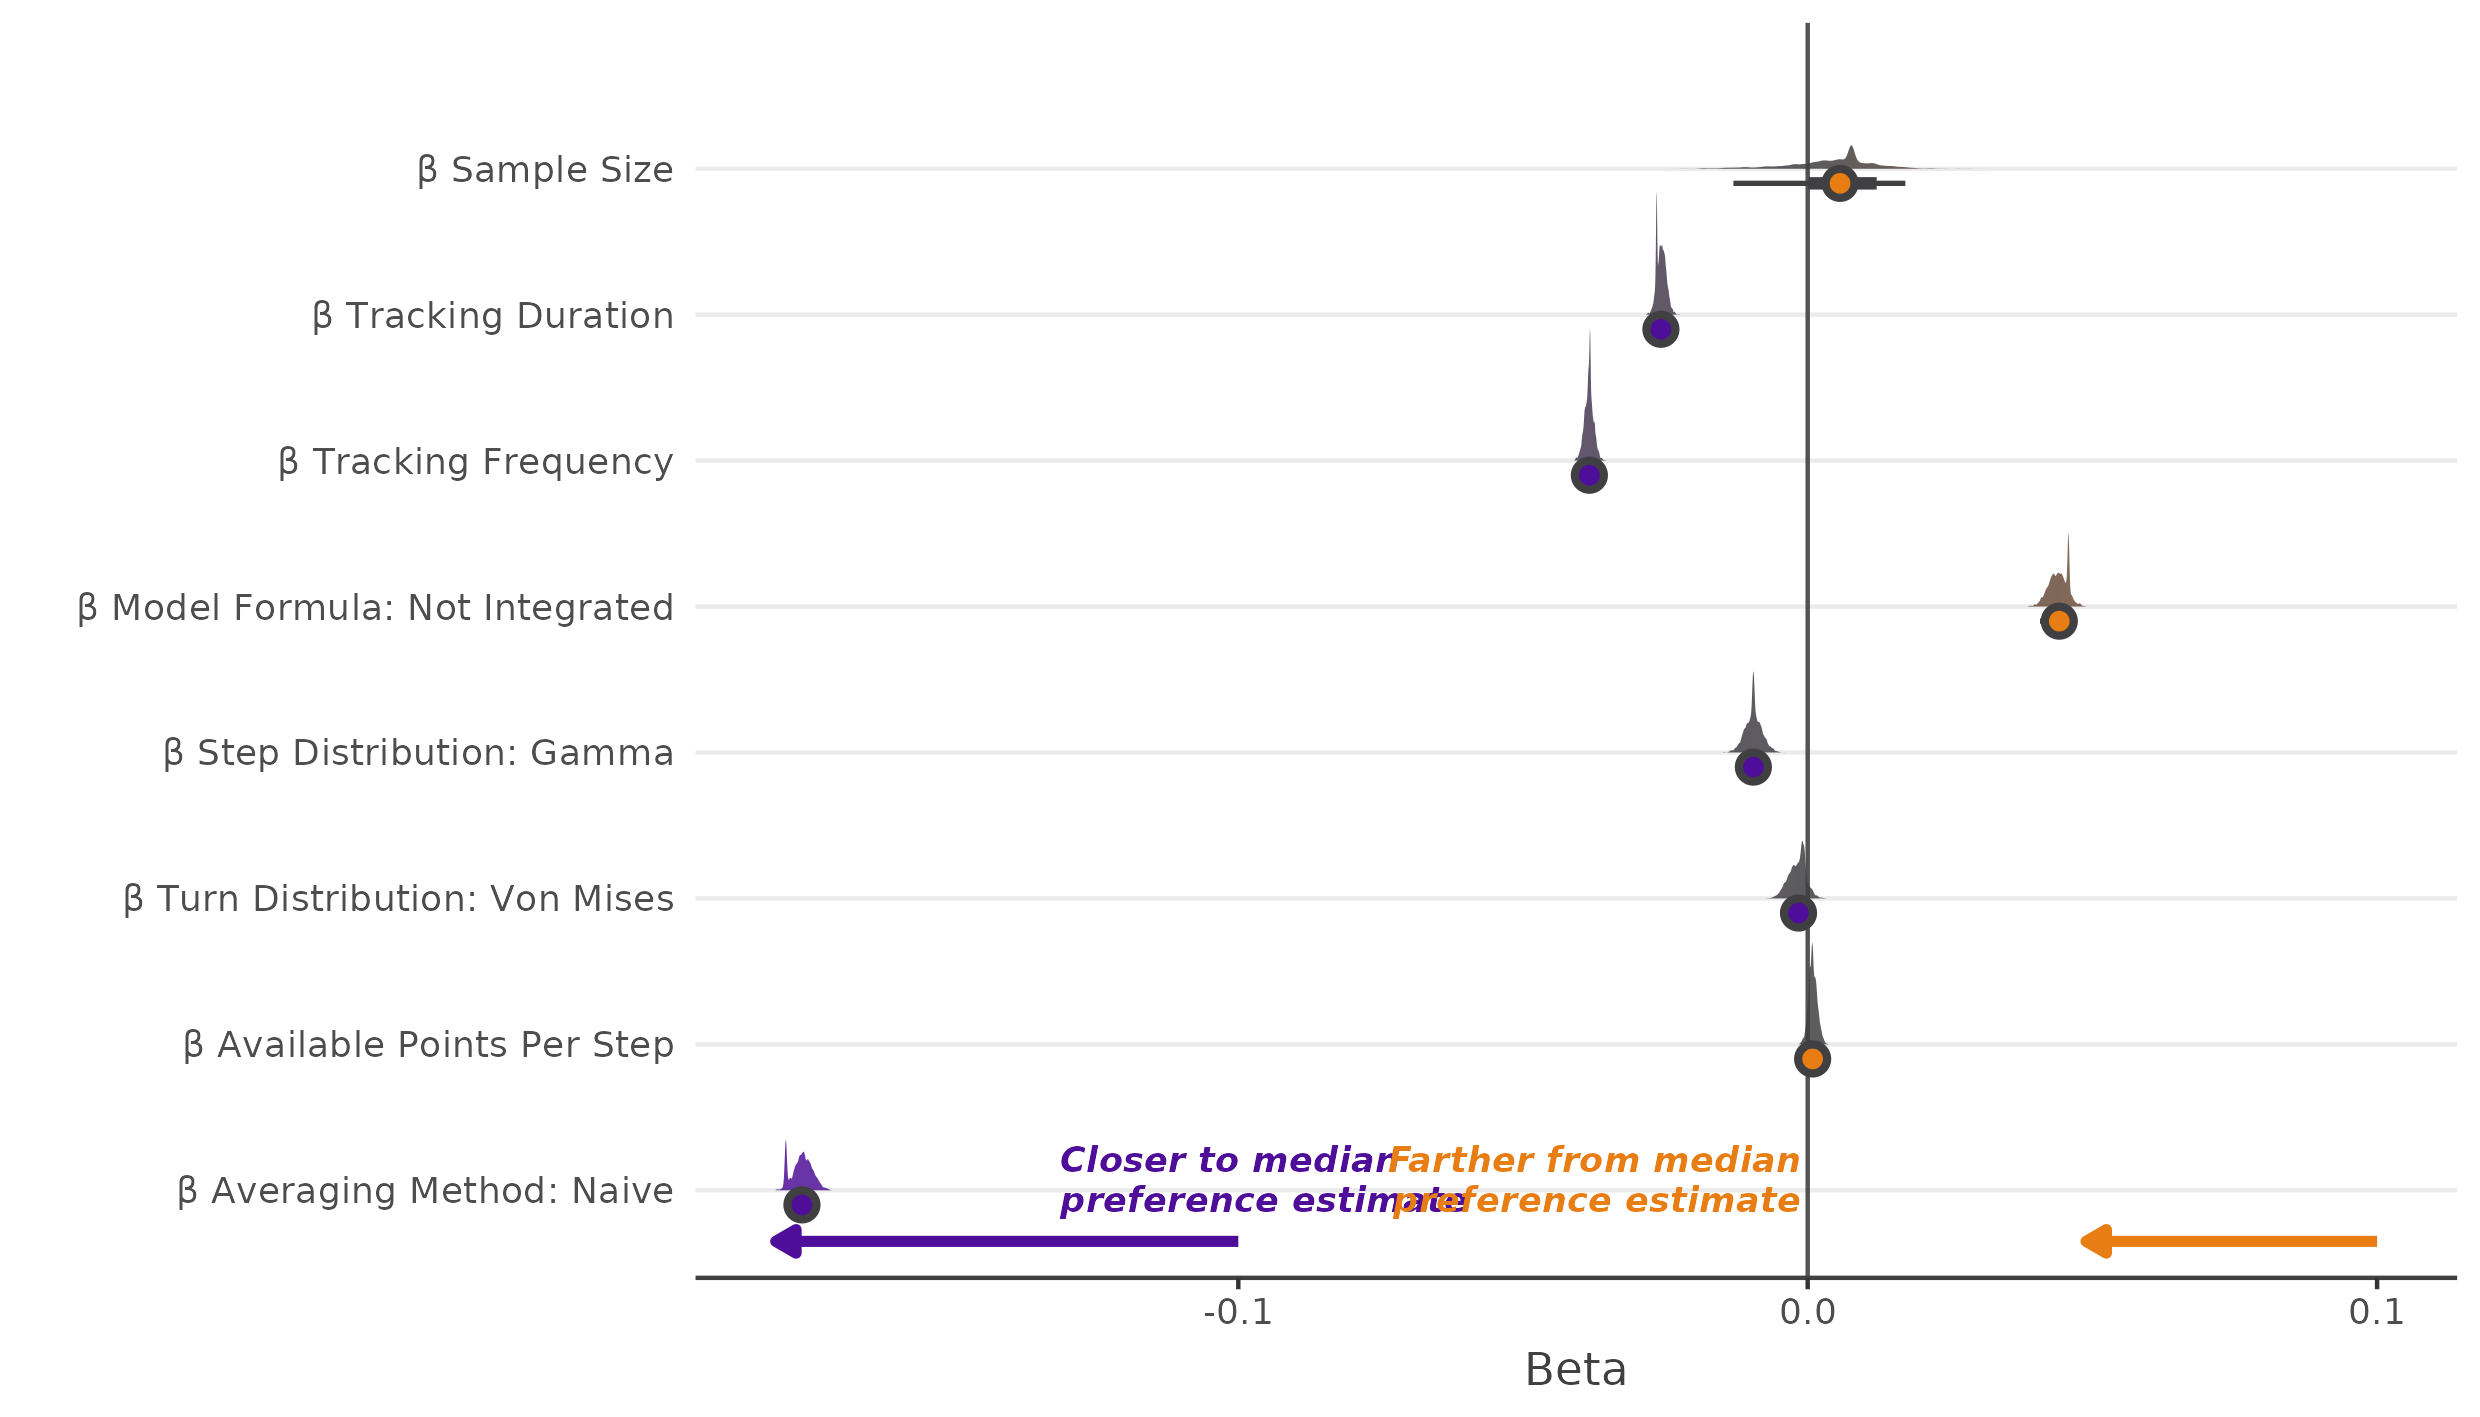
\includegraphics[width=1\linewidth]{../figures/ssfBrms_effectsPlot} \caption{Beta coefs}\label{fig:effectPlotSSF}
\end{figure}

\begin{figure}
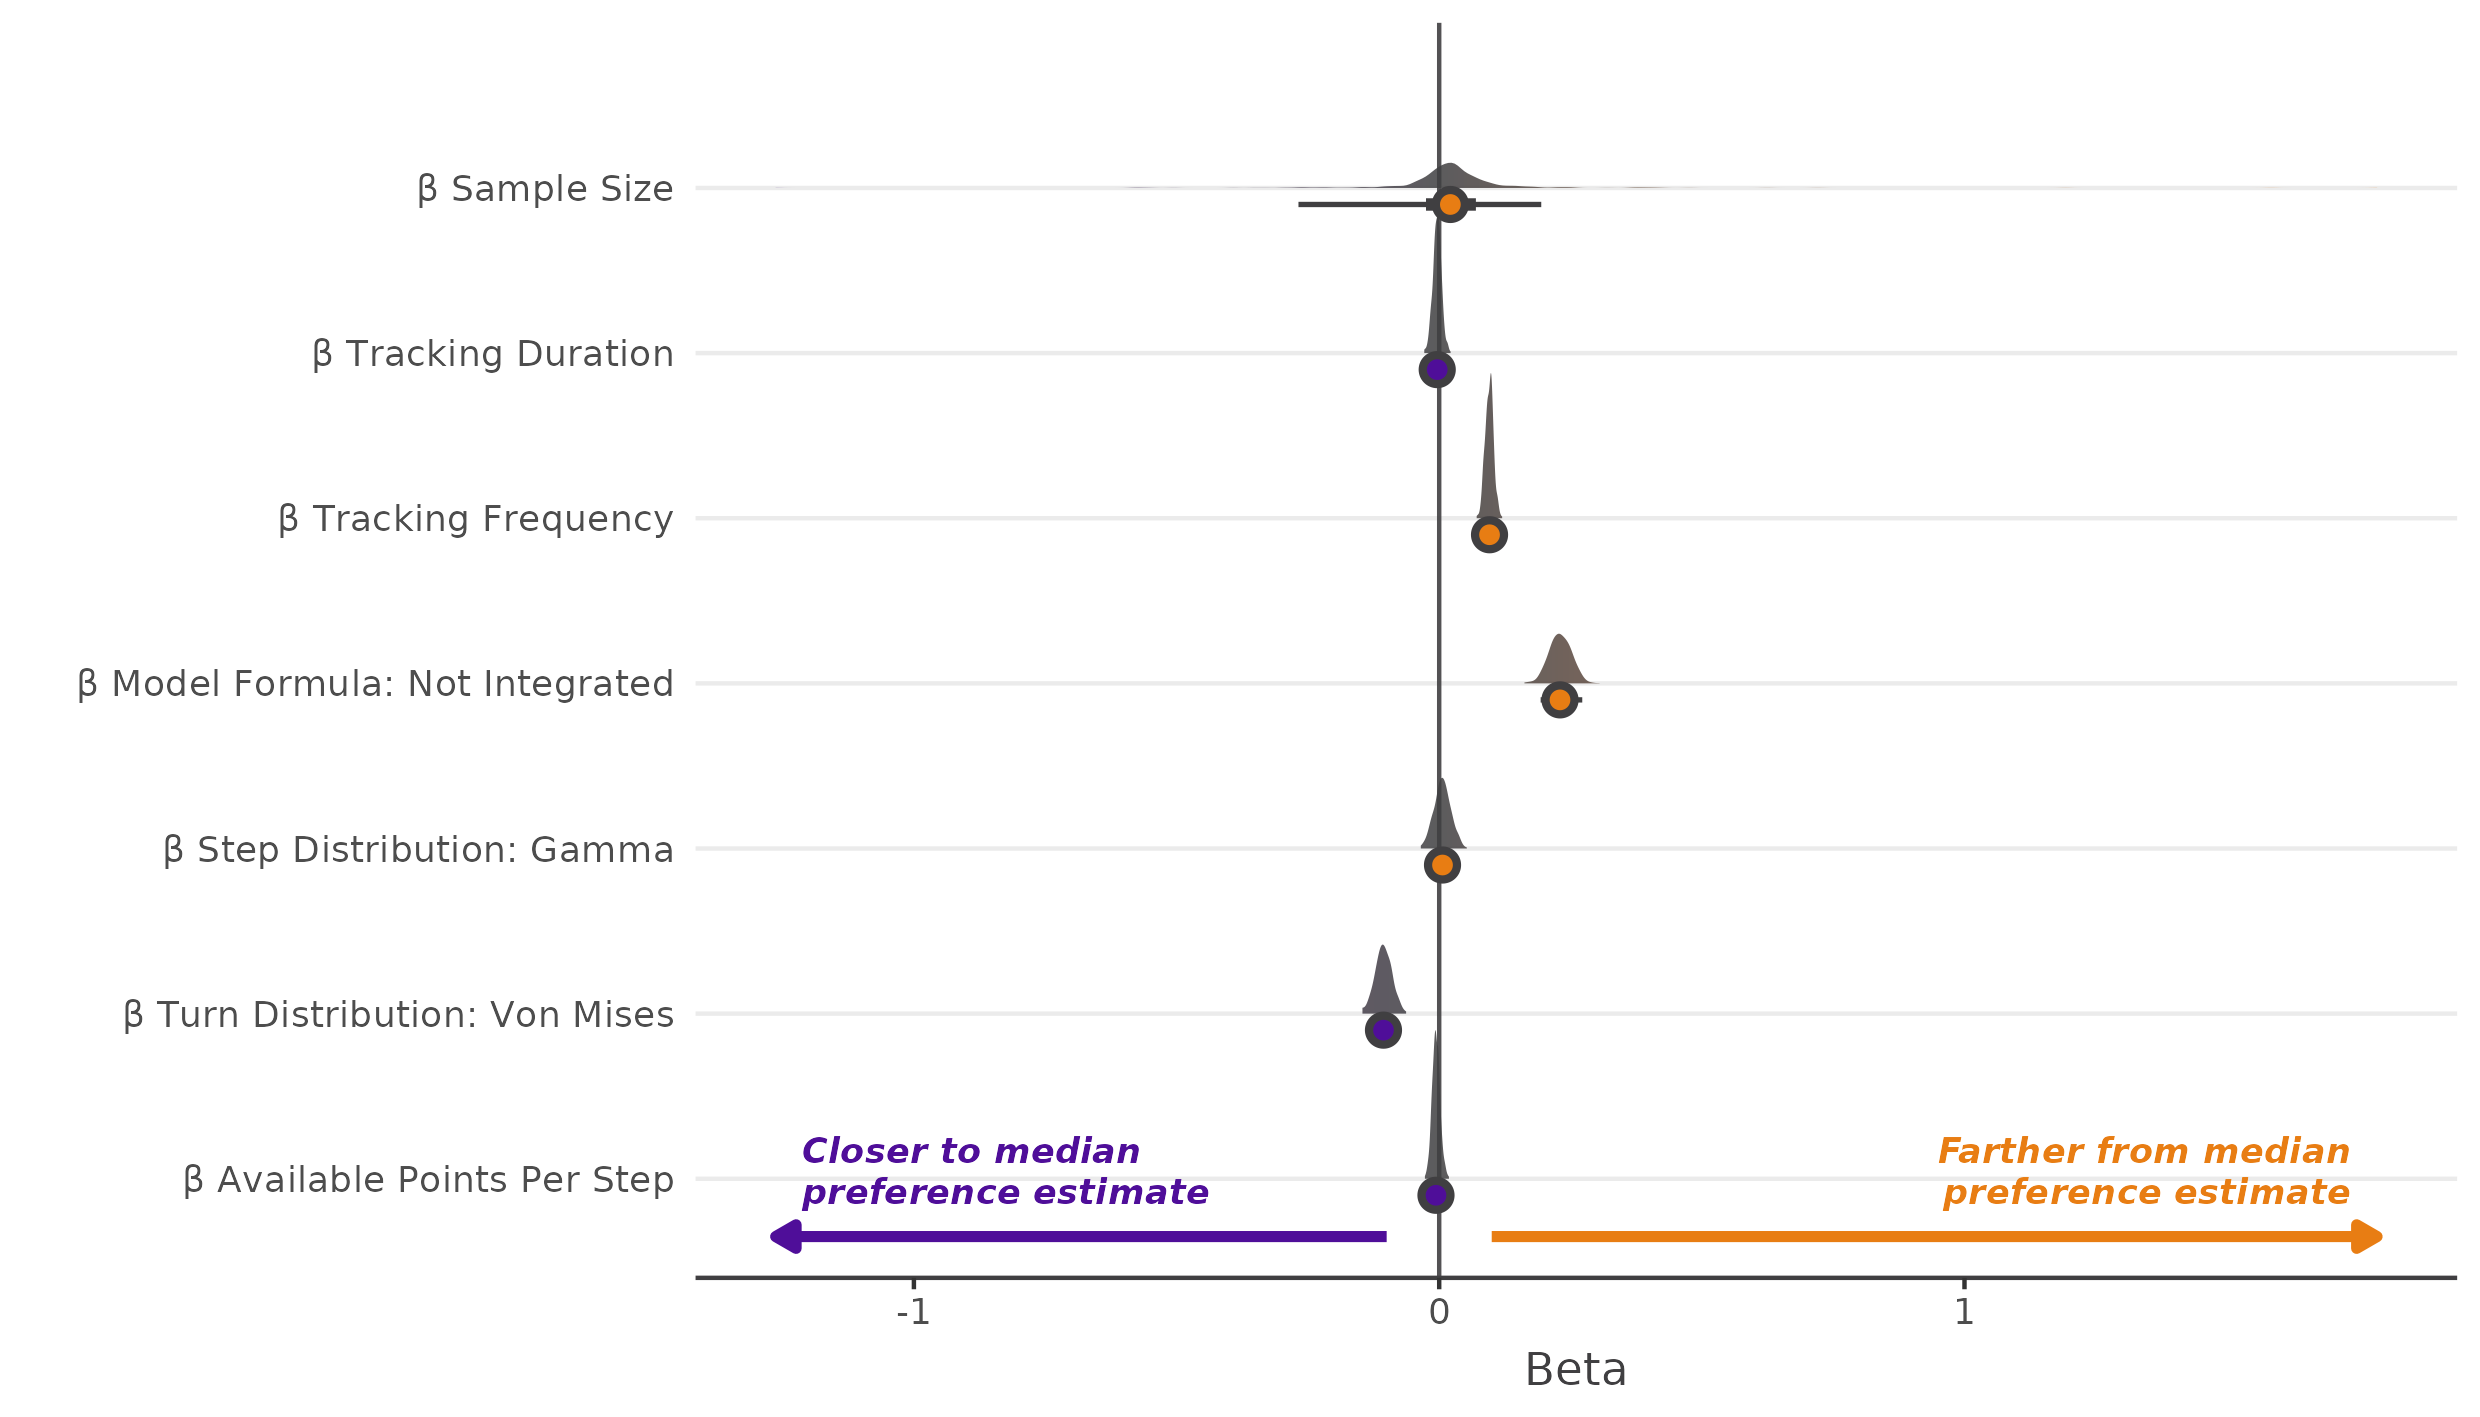
\includegraphics[width=1\linewidth]{../figures/twoStepBrms_effectsPlot} \caption{Beta coefs}\label{fig:effectPlotTwoStep}
\end{figure}

\begin{figure}
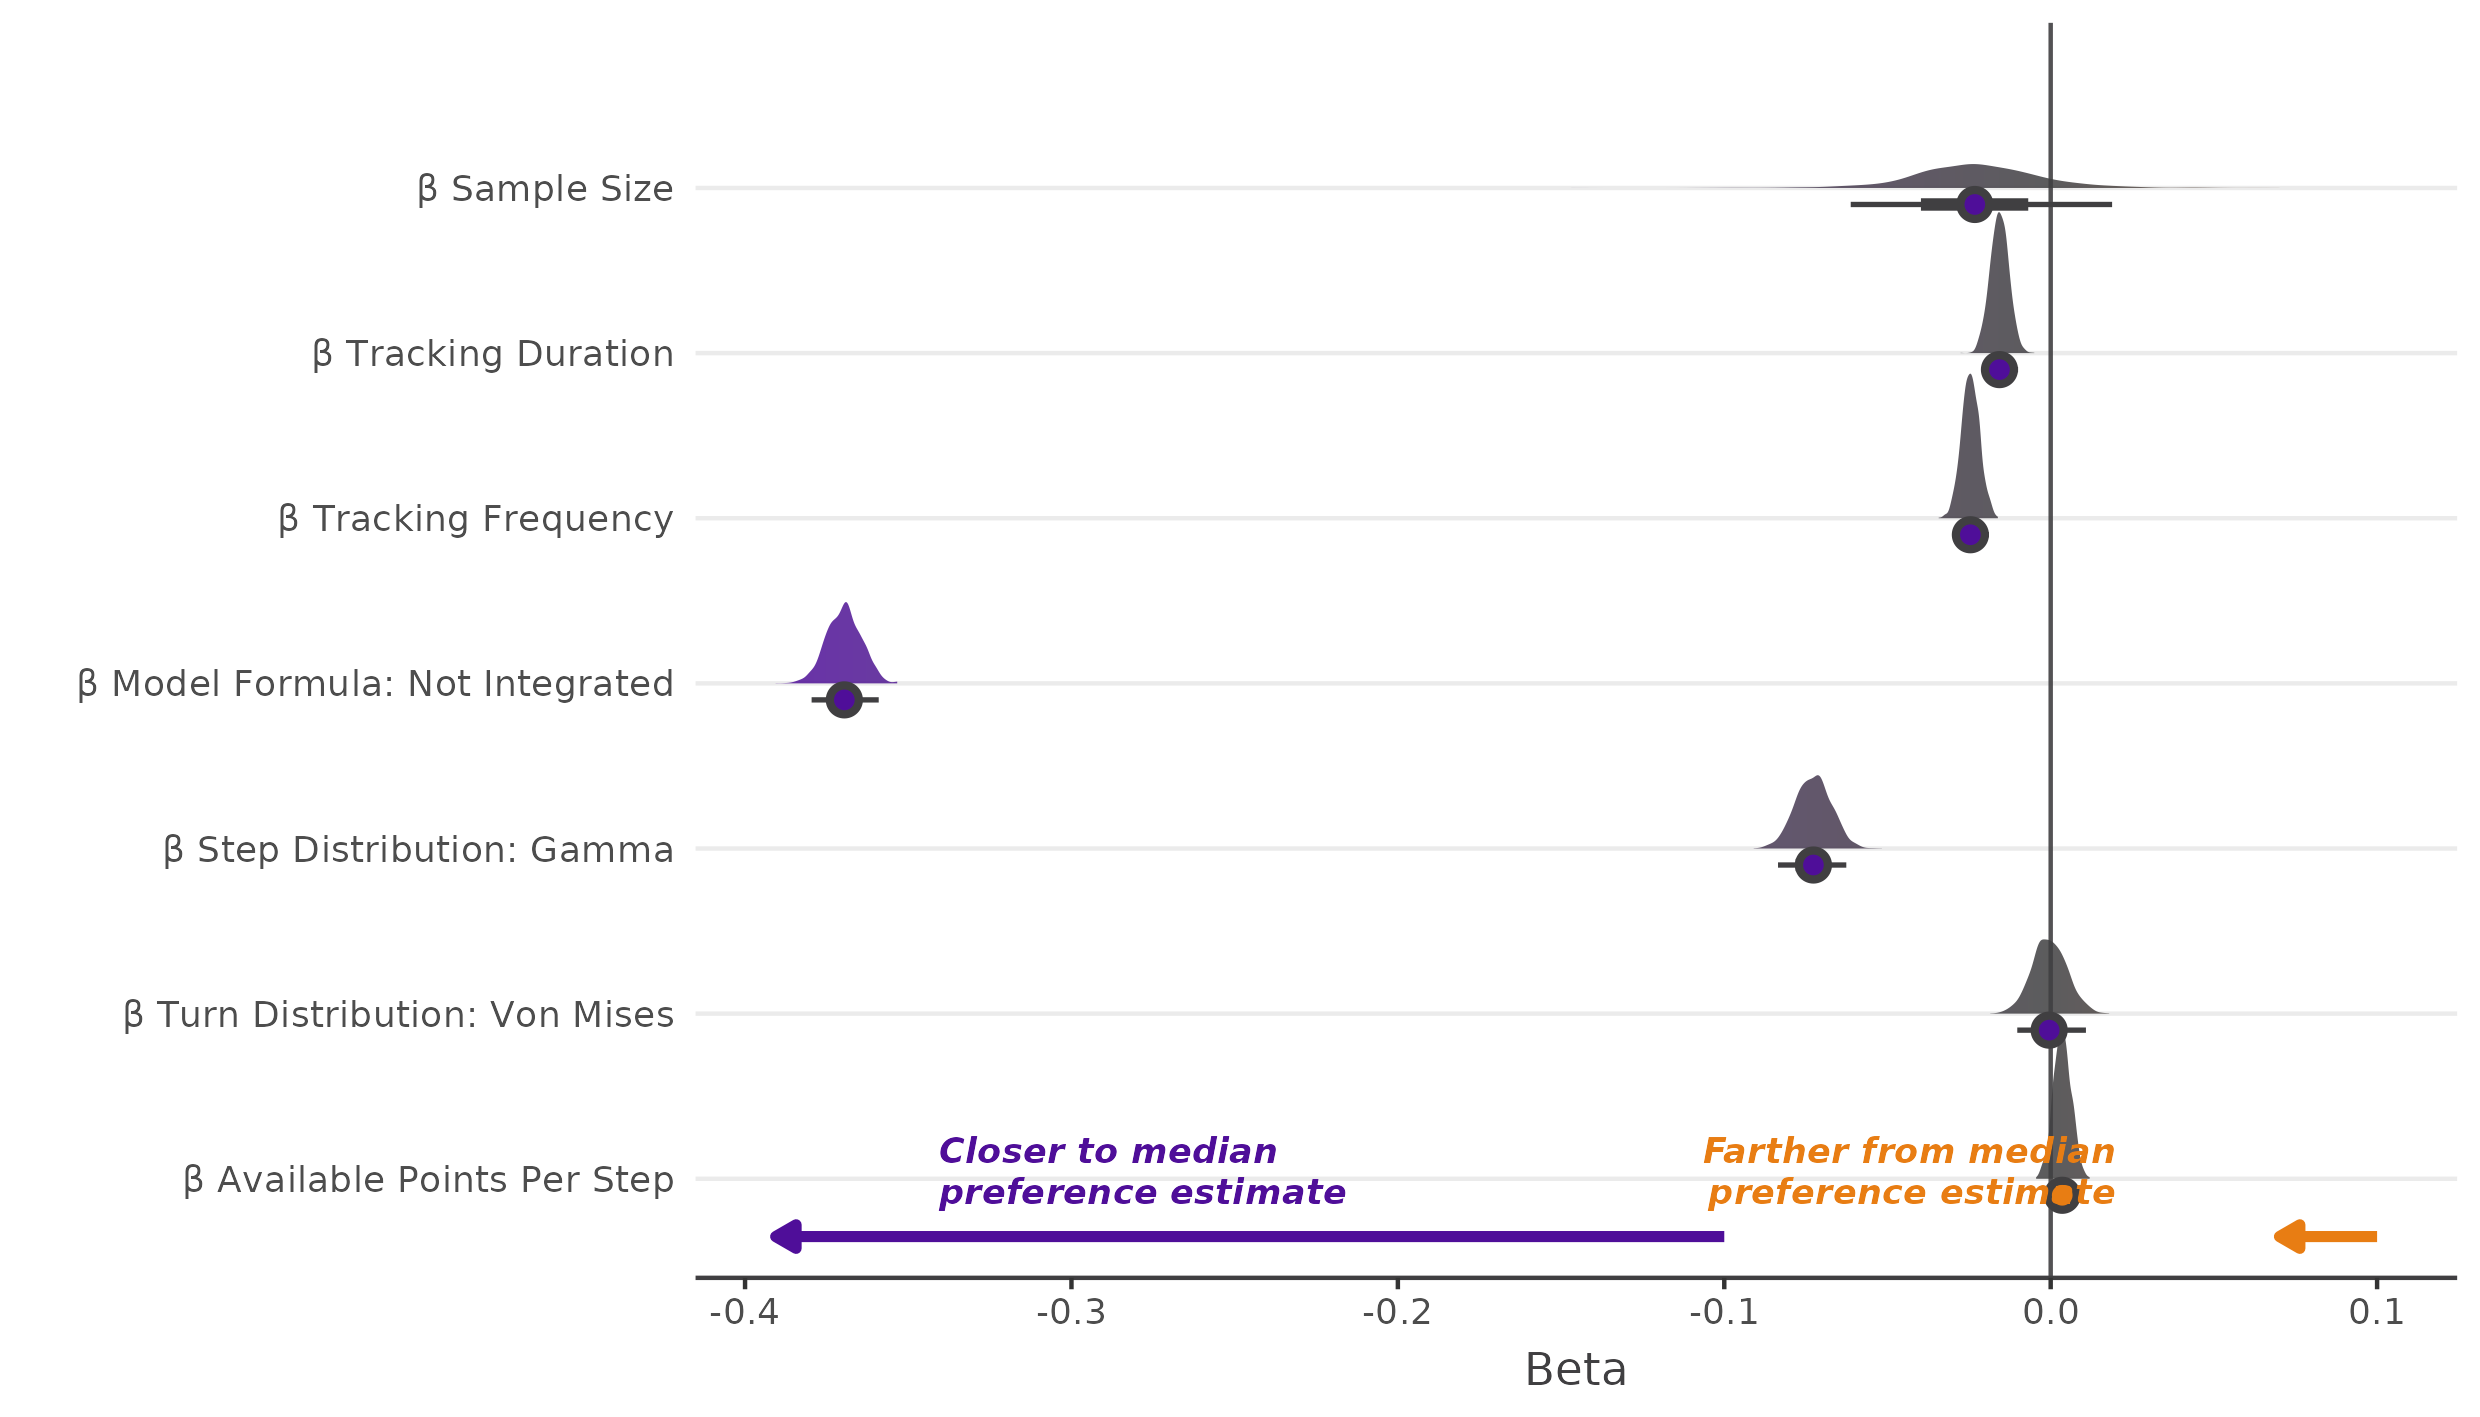
\includegraphics[width=1\linewidth]{../figures/poisBrms_effectsPlot} \caption{Beta coefs}\label{fig:effectPlotPois}
\end{figure}

\clearpage

\section*{References}\label{references}
\addcontentsline{toc}{section}{References}

\phantomsection\label{refs}
\begin{CSLReferences}{1}{0}
\bibitem[\citeproctext]{ref-rmarkdown2023}
Allaire J, Xie Y, Dervieux C, McPherson J, Luraschi J, Ushey K, Atkins A, Wickham H, Cheng J, Chang W, Iannone R. 2023. \emph{\href{https://github.com/rstudio/rmarkdown}{{rmarkdown}: Dynamic documents for r}}.

\bibitem[\citeproctext]{ref-auspurg_has_2021}
Auspurg K, Brüderl J. 2021. Has the {Credibility} of the {Social} {Sciences} {Been} {Credibly} {Destroyed}? {Reanalyzing} the {``{Many} {Analysts}, {One} {Data} {Set}''} {Project}. \emph{Socius: Sociological Research for a Dynamic World} 7:237802312110244. DOI: \href{https://doi.org/10.1177/23780231211024421}{10.1177/23780231211024421}.

\bibitem[\citeproctext]{ref-MuMIn}
Bartoń K. 2023. \emph{\href{https://CRAN.R-project.org/package=MuMIn}{MuMIn: Multi-model inference}}.

\bibitem[\citeproctext]{ref-barto_dissemination_2012}
Barto EK, Rillig MC. 2012. Dissemination biases in ecology: Effect sizes matter more than quality. \emph{Oikos} 121:228--235. DOI: \href{https://doi.org/10.1111/j.1600-0706.2011.19401.x}{10.1111/j.1600-0706.2011.19401.x}.

\bibitem[\citeproctext]{ref-bastiaansen_time_2020}
Bastiaansen JA, Kunkels YK, Blaauw FJ, Boker SM, Ceulemans E, Chen M, Chow S-M, Jonge P de, Emerencia AC, Epskamp S, Fisher AJ, Hamaker EL, Kuppens P, Lutz W, Meyer MJ, Moulder R, Oravecz Z, Riese H, Rubel J, Ryan O, Servaas MN, Sjobeck G, Snippe E, Trull TJ, Tschacher W, Veen DC van der, Wichers M, Wood PK, Woods WC, Wright AGC, Albers CJ, Bringmann LF. 2020. Time to get personal? {The} impact of researchers choices on the selection of treatment targets using the experience sampling methodology. \emph{Journal of Psychosomatic Research} 137:110211. DOI: \href{https://doi.org/10.1016/j.jpsychores.2020.110211}{10.1016/j.jpsychores.2020.110211}.

\bibitem[\citeproctext]{ref-sp}
Bivand RS, Pebesma E, Gomez-Rubio V. 2013. \emph{\href{https://asdar-book.org/}{Applied spatial data analysis with {R}, second edition}}. Springer, NY.

\bibitem[\citeproctext]{ref-Brembs2018}
Brembs B. 2018. Prestigious {Science} {Journals} {Struggle} to {Reach} {Even} {Average} {Reliability}. \emph{Frontiers in Human Neuroscience} 12:1--7. DOI: \href{https://doi.org/10.3389/fnhum.2018.00037}{10.3389/fnhum.2018.00037}.

\bibitem[\citeproctext]{ref-brms}
Bürkner P-C. 2021. Bayesian item response modeling in {R} with {brms} and {Stan}. \emph{Journal of Statistical Software} 100:1--54. DOI: \href{https://doi.org/10.18637/jss.v100.i05}{10.18637/jss.v100.i05}.

\bibitem[\citeproctext]{ref-adehabitatHS}
Calenge C, Mathieu Basille contributions from. 2023. \emph{\href{https://CRAN.R-project.org/package=adehabitatHS}{{adehabitatHS}: Analysis of habitat selection by animals}}.

\bibitem[\citeproctext]{ref-adehabitatHR}
Calenge C, Scott Fortmann-Roe contributions from. 2023. \emph{\href{https://CRAN.R-project.org/package=adehabitatHR}{{adehabitatHR}: Home range estimation}}.

\bibitem[\citeproctext]{ref-qs}
Ching T. 2023. \emph{\href{https://CRAN.R-project.org/package=qs}{{qs}: Quick serialization of r objects}}.

\bibitem[\citeproctext]{ref-TwoStepCLogit}
Craiu RV, Duchesne T, Fortin D, Baillargeon S. 2016. \emph{\href{https://CRAN.R-project.org/package=TwoStepCLogit}{TwoStepCLogit: Conditional logistic regression: A two-step estimation method}}.

\bibitem[\citeproctext]{ref-crane_lots_2021}
Crane M, Silva I, Marshall BM, Strine CT. 2021. Lots of movement, little progress: A review of reptile home range literature. \emph{PeerJ} 9:e11742. DOI: \href{https://doi.org/10.7717/peerj.11742}{10.7717/peerj.11742}.

\bibitem[\citeproctext]{ref-desbureaux_subjective_2021}
Desbureaux S. 2021. Subjective modeling choices and the robustness of impact evaluations in conservation science. \emph{Conservation Biology} 35:1615--1626. DOI: \href{https://doi.org/10.1111/cobi.13728}{10.1111/cobi.13728}.

\bibitem[\citeproctext]{ref-devezer_case_2021}
Devezer B, Navarro DJ, Vandekerckhove J, Ozge Buzbas E. 2021. The case for formal methodology in scientific reform. \emph{Royal Society Open Science} 8:rsos.200805, 200805. DOI: \href{https://doi.org/10.1098/rsos.200805}{10.1098/rsos.200805}.

\bibitem[\citeproctext]{ref-doherty_coupling_2018}
Doherty TS, Driscoll DA. 2018. Coupling movement and landscape ecology for animal conservation in production landscapes. \emph{Proceedings of the Royal Society B: Biological Sciences} 285:20172272. DOI: \href{https://doi.org/10.1098/rspb.2017.2272}{10.1098/rspb.2017.2272}.

\bibitem[\citeproctext]{ref-doherty_animal_2019}
Doherty TS, Fist CN, Driscoll DA. 2019. Animal movement varies with resource availability, landscape configuration and body size: A conceptual model and empirical example. \emph{Landscape Ecology} 34:603--614. DOI: \href{https://doi.org/10.1007/s10980-019-00795-x}{10.1007/s10980-019-00795-x}.

\bibitem[\citeproctext]{ref-fanelli_pressures_2010}
Fanelli D. 2010. Do {Pressures} to {Publish} {Increase} {Scientists}' {Bias}? {An} {Empirical} {Support} from {US} {States} {Data}. \emph{PLoS ONE} 5:e10271. DOI: \href{https://doi.org/10.1371/journal.pone.0010271}{10.1371/journal.pone.0010271}.

\bibitem[\citeproctext]{ref-ctmm}
Fleming CH, Calabrese JM. 2023. \emph{{ctmm}: Continuous-time movement modeling}.

\bibitem[\citeproctext]{ref-forstmeier_detecting_2017}
Forstmeier W, Wagenmakers E-J, Parker TH. 2017. Detecting and avoiding likely false-positive findings -- a practical guide: {Avoiding} false-positive findings. \emph{Biological Reviews} 92:1941--1968. DOI: \href{https://doi.org/10.1111/brv.12315}{10.1111/brv.12315}.

\bibitem[\citeproctext]{ref-grateful}
Francisco Rodríguez-Sánchez, Connor P. Jackson, Shaurita D. Hutchins. 2023. \emph{\href{https://github.com/Pakillo/grateful}{{grateful}: Facilitate citation of r packages}}.

\bibitem[\citeproctext]{ref-fraser_role_2020}
Fraser H, Barnett A, Parker TH, Fidler F. 2020. The role of replication studies in ecology. \emph{Ecology and Evolution} 10:5197--5207. DOI: \href{https://doi.org/10.1002/ece3.6330}{10.1002/ece3.6330}.

\bibitem[\citeproctext]{ref-Fraser2018}
Fraser KC, Davies KT, Davy CM, Ford AT, Flockhart DTT, Martins EG. 2018. Tracking the conservation promise of movement ecology. \emph{Frontiers in Ecology and Evolution} 6:150. DOI: \href{https://doi.org/10.3389/FEVO.2018.00150}{10.3389/FEVO.2018.00150}.

\bibitem[\citeproctext]{ref-freedman_economics_2015}
Freedman LP, Cockburn IM, Simcoe TS. 2015. The {Economics} of {Reproducibility} in {Preclinical} {Research}. \emph{PLOS Biology} 13:e1002165. DOI: \href{https://doi.org/10.1371/journal.pbio.1002165}{10.1371/journal.pbio.1002165}.

\bibitem[\citeproctext]{ref-bayesplot}
Gabry J, Simpson D, Vehtari A, Betancourt M, Gelman A. 2019. Visualization in bayesian workflow. \emph{J. R. Stat. Soc. A} 182:389--402. DOI: \href{https://doi.org/10.1111/rssa.12378}{10.1111/rssa.12378}.

\bibitem[\citeproctext]{ref-gelman_garden_2013}
Gelman A, Loken E. 2013. \href{http://www.stat.columbia.edu/~gelman/research/unpublished/p_hacking.pdf}{The garden of forking paths: {Why} multiple comparisons can be a problem, even when there is no "fishing expedition" or "p-hacking" and the research hypothesis was posited ahead of time}. :17.

\bibitem[\citeproctext]{ref-gould_same_2023}
Gould E, Fraser H, Parker T, Nakagawa S, Griffith S, Vesk P, Fidler F, Abbey-Lee R, Abbott J, Aguirre L, Alcaraz C, Altschul D, Arekar K, Atkins J, Atkinson J, Barrett M, Bell K, Bello S, Berauer B, Bertram M, Billman P, Blake C, Blake S, Bliard L, Bonisoli-Alquati A, Bonnet T, Bordes C, Bose A, Botterill-James T, Boyd M, Boyle S, Bradfer-Lawrence T, Brand J, Brengdahl M, Bulla M, Bussière L, Camerlenghi E, Campbell S, Campos L, Caravaggi A, Cardoso P, Carroll C, Catanach T, Chen X, Chik HYJ, Choy E, Christie A, Chuang A, Chunco A, Clark B, Cox M, Cressman K, Crouch C, D'Amelio P, De Sousa A, Döbert T, Dobler R, Dobson A, Doherty T, Drobniak S, Duffy A, Dunn R, Dunning J, Eberhart-Hertel L, Elmore J, Elsherif M, English H, Ensminger D, Ernst U, Ferguson S, Ferreira-Arruda T, Fieberg J, Finch E, Fiorenza E, Fisher D, Forstmeier W, Fourcade Y, Francesca Santostefano F, Frank G, Freund C, Gandy S, Gannon D, García-Cervigón A, Géron C, Gilles M, Girndt A, Gliksman D, Goldspiel H, Gomes D, Goslee S, Gosnell J, Gratton P, Grebe N, Greenler S, Griffith D, Griffith F, Grossman J, Güncan A, Haesen S, Hagan J, Harrison N, Hasnain S, Havird J, Heaton A, Hsu B-Y, Iranzo E, Iverson E, Jimoh S, Johnson D, Johnsson M, Jorna J, Jucker T, Jung M, Kačergytė I, Ke A, Kelly C, Keogan K, Keppeler F, Killion A, Kim D, Kochan D, Korsten P, Kothari S, Kuppler J, Kusch J, Lagisz M, Larkin D, Larson C, Lauck K, Lauterbur M, Law A, Léandri-Breton D-J, Lievens E, Lima D, Lindsay S, Macphie K, Mair M, Malm L, Mammola S, Manhart M, Mäntylä E, Marchand P, Marshall B, Martin D, Martin J, Martin C, Martinig A, McCallum E, McNew S, Meiners S, Michelangeli M, Moiron M, Moreira B, Mortensen J, Mos B, Muraina T, Nelli L, Nilsonne G, Nolazco S, Nooten S, Novotny J, Olin A, Organ C, Ostevik K, Palacio F, Paquet M, Pascall D, Pasquarella V, Payo-Payo A, Pedersen K, Perez G, Perry K, Pottier P, Proulx M, Proulx R, Pruett J, Ramananjato V, Randimbiarison F, Razafindratsima O, Rennison D, Riva F, Riyahi S, Roast M, Rocha F, Roche D, Román-Palacios C, Rosenberg M, Ross J, Rowland F, Rugemalila D, Russell A, Ruuskanen S, Saccone P, Sadeh A, Salazar S, Sales K, Salmón P, Sanchez-Tojar A, Santos L, Schilling H, Schmidt M, Schmoll T, Schneider A, Schrock A, Schroeder J, Schtickzelle N, Schultz N, Scott D, Shapiro J, Sharma N, Shearer C, Sitvarin M, Skupien F, Slinn H, Smith J, Smith G, Sollmann R, Stack Whitney K, Still S, Stuber E, Sutton G, Swallow B, Taff C, Takola E, Tanentzap A, Thawley C, Tortorelli C, Trlica A, Turnell B, Urban L, Van De Vondel S, Van Oordt F, Vanderwel M, Vanderwel K, Vanderwolf K, Verrelli B, Vieira M, Vollering J, Walker X, Walter J, Waryszak P, Weaver R, Weller D, Whelan S, White R, Wolfson D, Wood A, Yanco S, Yen J, Youngflesh C, Zilio G, Zimmer C, Zitomer R, Villamil N, Tompkins E. 2023. Same data, different analysts: Variation in effect sizes due to analytical decisions in ecology and evolutionary biology. \emph{EcoEvoRxiv}. DOI: \href{https://doi.org/10.32942/X2GG62}{10.32942/X2GG62}.

\bibitem[\citeproctext]{ref-raster}
Hijmans RJ. 2023. \emph{\href{https://CRAN.R-project.org/package=raster}{{raster}: Geographic data analysis and modeling}}.

\bibitem[\citeproctext]{ref-homberger_strong_2021}
Homberger B, Jenni L, Duplain J, Lanz M, Schaub M. 2021. Strong effects of radio-tags, social group and release date on survival of reintroduced grey partridges. \emph{Animal Conservation} 24:677--688. DOI: \href{https://doi.org/10.1111/acv.12673}{10.1111/acv.12673}.

\bibitem[\citeproctext]{ref-huntingtonklein_influence_2021}
Huntington‐Klein N, Arenas A, Beam E, Bertoni M, Bloem JR, Burli P, Chen N, Grieco P, Ekpe G, Pugatch T, Saavedra M, Stopnitzky Y. 2021. The influence of hidden researcher decisions in applied microeconomics. \emph{Economic Inquiry} 59:944--960. DOI: \href{https://doi.org/10.1111/ecin.12992}{10.1111/ecin.12992}.

\bibitem[\citeproctext]{ref-jennions_relationships_2002}
Jennions MD, Møller AP. 2002. Relationships fade with time: A meta-analysis of temporal trends in publication in ecology and evolution. \emph{Proceedings of the Royal Society of London. Series B: Biological Sciences} 269:43--48. DOI: \href{https://doi.org/10.1098/rspb.2001.1832}{10.1098/rspb.2001.1832}.

\bibitem[\citeproctext]{ref-ggdist}
Kay M. 2023a. \emph{{ggdist}: Visualizations of distributions and uncertainty}. DOI: \href{https://doi.org/10.5281/zenodo.3879620}{10.5281/zenodo.3879620}.

\bibitem[\citeproctext]{ref-tidybayes}
Kay M. 2023b. \emph{{tidybayes}: Tidy data and geoms for {Bayesian} models}. DOI: \href{https://doi.org/10.5281/zenodo.1308151}{10.5281/zenodo.1308151}.

\bibitem[\citeproctext]{ref-kelly_rate_2019}
Kelly CD. 2019. Rate and success of study replication in ecology and evolution. \emph{PeerJ} 7:e7654. DOI: \href{https://doi.org/10.7717/peerj.7654}{10.7717/peerj.7654}.

\bibitem[\citeproctext]{ref-kourounis_towards_2018}
Kourounis D, Fuchs A, Schenk O. 2018. \href{https://doi.org/10.1109/TPWRS.2017.2789187}{Towards the next generation of multiperiod optimal power flow solvers}. \emph{IEEE Transactions on Power Systems} PP:1--10.

\bibitem[\citeproctext]{ref-move}
Kranstauber B, Smolla M, Scharf AK. 2023. \emph{\href{https://CRAN.R-project.org/package=move}{{move}: Visualizing and analyzing animal track data}}.

\bibitem[\citeproctext]{ref-tarchetypes}
Landau WM. 2021b. \emph{Tarchetypes: Archetypes for targets}.

\bibitem[\citeproctext]{ref-targets}
Landau WM. 2021a. \href{https://doi.org/10.21105/joss.02959}{The targets r package: A dynamic make-like function-oriented pipeline toolkit for reproducibility and high-performance computing}. \emph{Journal of Open Source Software} 6:2959.

\bibitem[\citeproctext]{ref-lindgren_explicit_2011}
Lindgren F, Rue H, Lindström J. 2011. An explicit link between {Gaussian} fields and {Gaussian} {Markov} random fields: The stochastic partial differential equation approach (with discussion). \emph{Journal of the Royal Statistical Society B} 73:423--498.

\bibitem[\citeproctext]{ref-performance}
Lüdecke D, Ben-Shachar MS, Patil I, Waggoner P, Makowski D. 2021. {performance}: An {R} package for assessment, comparison and testing of statistical models. \emph{Journal of Open Source Software} 6:3139. DOI: \href{https://doi.org/10.21105/joss.03139}{10.21105/joss.03139}.

\bibitem[\citeproctext]{ref-abmAnimalMovement}
Marshall BM, Duthie AB. 2022. \href{https://0}{{abmAnimalMovement}: An r package for simulating animal movement using an agent-based model}. \emph{F1000} 0:0.

\bibitem[\citeproctext]{ref-martins_bayesian_2013}
Martins TG, Simpson D, Lindgren F, Rue H. 2013. Bayesian computing with {INLA}: {N}ew features. \emph{Computational Statistics and Data Analysis} 67:68--83.

\bibitem[\citeproctext]{ref-mueller_how_2011}
Mueller T, Olson KA, Dressler G, Leimgruber P, Fuller TK, Nicolson C, Novaro AJ, Bolgeri MJ, Wattles D, DeStefano S, Calabrese JM, Fagan WF. 2011. How landscape dynamics link individual- to population-level movement patterns: A multispecies comparison of ungulate relocation data: {Population}-level movement patterns. \emph{Global Ecology and Biogeography} 20:683--694. DOI: \href{https://doi.org/10.1111/j.1466-8238.2010.00638.x}{10.1111/j.1466-8238.2010.00638.x}.

\bibitem[\citeproctext]{ref-muff_accounting_2020}
Muff S, Signer J, Fieberg J. 2020. Accounting for individual-specific variation in habitat-selection studies: Efficient estimation of mixed-effects models using bayesian or frequentist computation. \emph{Journal of Animal Ecology} 89:80--92. DOI: \href{https://doi.org/10.1111/1365-2656.13087}{10.1111/1365-2656.13087}.

\bibitem[\citeproctext]{ref-here}
Müller K. 2020. \emph{\href{https://CRAN.R-project.org/package=here}{{here}: A simpler way to find your files}}.

\bibitem[\citeproctext]{ref-tibble}
Müller K, Wickham H. 2023. \emph{\href{https://CRAN.R-project.org/package=tibble}{{tibble}: Simple data frames}}.

\bibitem[\citeproctext]{ref-nakagawa_replicating_2015}
Nakagawa S, Parker TH. 2015. Replicating research in ecology and evolution: Feasibility, incentives, and the cost-benefit conundrum. \emph{BMC Biology} 13:88. DOI: \href{https://doi.org/10.1186/s12915-015-0196-3}{10.1186/s12915-015-0196-3}.

\bibitem[\citeproctext]{ref-open_science_collaboration_estimating_2015}
Open Science Collaboration. 2015. Estimating the reproducibility of psychological science. \emph{Science} 349:aac4716--aac4716. DOI: \href{https://doi.org/10.1126/science.aac4716}{10.1126/science.aac4716}.

\bibitem[\citeproctext]{ref-palmer_quasi-replication_2000}
Palmer AR. 2000. Quasi-{Replication} and the {Contract} of {Error}: {Lessons} from {Sex} {Ratios}, {Heritabilities} and {Fluctuating} {Asymmetry}. \emph{Annual Review of Ecology and Systematics} 31:441--480. DOI: \href{https://doi.org/10.1146/annurev.ecolsys.31.1.441}{10.1146/annurev.ecolsys.31.1.441}.

\bibitem[\citeproctext]{ref-parker_what_2013}
Parker TH. 2013. What do we really know about the signalling role of plumage colour in blue tits? {A} case study of impediments to progress in evolutionary biology: {Case} study of impediments to progress. \emph{Biological Reviews} 88:511--536. DOI: \href{https://doi.org/10.1111/brv.12013}{10.1111/brv.12013}.

\bibitem[\citeproctext]{ref-patchwork}
Pedersen TL. 2022. \emph{\href{https://CRAN.R-project.org/package=patchwork}{Patchwork: The composer of plots}}.

\bibitem[\citeproctext]{ref-portugal_externally_2022}
Portugal SJ, White CR. 2022. Externally attached biologgers cause compensatory body mass loss in birds. \emph{Methods in Ecology and Evolution} 13:294--302. DOI: \href{https://doi.org/10.1111/2041-210X.13754}{10.1111/2041-210X.13754}.

\bibitem[\citeproctext]{ref-base}
R Core Team. 2023. \emph{\href{https://www.R-project.org/}{R: A language and environment for statistical computing}}. Vienna, Austria: R Foundation for Statistical Computing.

\bibitem[\citeproctext]{ref-rijnhart_assessing_2021}
Rijnhart JJM, Twisk JWR, Deeg DJH, Heymans MW. 2021. Assessing the {Robustness} of {Mediation} {Analysis} {Results} {Using} {Multiverse} {Analysis}. \emph{Prevention Science}. DOI: \href{https://doi.org/10.1007/s11121-021-01280-1}{10.1007/s11121-021-01280-1}.

\bibitem[\citeproctext]{ref-rstudio}
RStudio Team. 2022. \emph{\href{http://www.rstudio.com/}{{RStudio}: Integrated development environment for r}}. Boston, MA: RStudio, PBC.

\bibitem[\citeproctext]{ref-rue_approximate_2009}
Rue H, Martino S, Chopin N. 2009. Approximate {Bayesian} inference for latent {Gaussian} models using integrated nested {Laplace} approximations (with discussion). \emph{Journal of the Royal Statistical Society B} 71:319--392.

\bibitem[\citeproctext]{ref-rue_bayesian_2017}
Rue H, Riebler AI, Sørbye SH, Illian JB, Simpson DP, Lindgren FK. 2017. \href{http://arxiv.org/abs/1604.00860}{Bayesian computing with {INLA}: {A} review}. \emph{Annual Reviews of Statistics and Its Applications} 4:395--421.

\bibitem[\citeproctext]{ref-salis_how_2021}
Salis A, Lena J-P, Lengagne T. 2021. How {Subtle} {Protocol} {Choices} {Can} {Affect} {Biological} {Conclusions}: {Great} {Tits}' {Response} to {Allopatric} {Mobbing} {Calls}. \emph{Animal Behavior and Cognition} 8:152--165. DOI: \href{https://doi.org/10.26451/abc.08.02.05.2021}{10.26451/abc.08.02.05.2021}.

\bibitem[\citeproctext]{ref-sanchez-tojar_meta-analysis_2018}
Sánchez-Tójar A, Nakagawa S, Sánchez-Fortún M, Martin DA, Ramani S, Girndt A, Bókony V, Kempenaers B, Liker A, Westneat DF, Burke T, Schroeder J. 2018. Meta-analysis challenges a textbook example of status signalling and demonstrates publication bias. \emph{eLife} 7:e37385. DOI: \href{https://doi.org/10.7554/eLife.37385}{10.7554/eLife.37385}.

\bibitem[\citeproctext]{ref-RandomFields}
Schlather M, Malinowski A, Menck PJ, Oesting M, Strokorb K. 2015. \href{https://www.jstatsoft.org/v63/i08/}{Analysis, simulation and prediction of multivariate random fields with package {RandomFields}}. \emph{Journal of Statistical Software} 63:1--25.

\bibitem[\citeproctext]{ref-NLMR}
Sciaini M, Fritsch M, Scherer C, Simpkins CE. 2018. \href{https://doi.org/10.1111/2041-210X.13076}{NLMR and landscapetools: An integrated environment for simulating and modifying neutral landscape models in r}. \emph{Methods in Ecololgy and Evolution} 00:1--9.

\bibitem[\citeproctext]{ref-seguin_no_2012}
Seguin A, Forstmeier W. 2012. No {Band} {Color} {Effects} on {Male} {Courtship} {Rate} or {Body} {Mass} in the {Zebra} {Finch}: {Four} {Experiments} and a {Meta}-{Analysis}. \emph{PLoS ONE} 7:e37785. DOI: \href{https://doi.org/10.1371/journal.pone.0037785}{10.1371/journal.pone.0037785}.

\bibitem[\citeproctext]{ref-amt}
Signer J, Fieberg J, Avgar T. 2019. Animal movement tools (amt): R package for managing tracking data and conducting habitat selection analyses. \emph{Ecology and Evolution} 9:880--890.

\bibitem[\citeproctext]{ref-silberzahn_many_2018}
Silberzahn R, Uhlmann EL, Martin DP, Anselmi P, Aust F, Awtrey E, Bahník Š, Bai F, Bannard C, Bonnier E, Carlsson R, Cheung F, Christensen G, Clay R, Craig MA, Dalla Rosa A, Dam L, Evans MH, Flores Cervantes I, Fong N, Gamez-Djokic M, Glenz A, Gordon-McKeon S, Heaton TJ, Hederos K, Heene M, Hofelich Mohr AJ, Högden F, Hui K, Johannesson M, Kalodimos J, Kaszubowski E, Kennedy DM, Lei R, Lindsay TA, Liverani S, Madan CR, Molden D, Molleman E, Morey RD, Mulder LB, Nijstad BR, Pope NG, Pope B, Prenoveau JM, Rink F, Robusto E, Roderique H, Sandberg A, Schlüter E, Schönbrodt FD, Sherman MF, Sommer SA, Sotak K, Spain S, Spörlein C, Stafford T, Stefanutti L, Tauber S, Ullrich J, Vianello M, Wagenmakers E-J, Witkowiak M, Yoon S, Nosek BA. 2018. Many {Analysts}, {One} {Data} {Set}: {Making} {Transparent} {How} {Variations} in {Analytic} {Choices} {Affect} {Results}. \emph{Advances in Methods and Practices in Psychological Science} 1:337--356. DOI: \href{https://doi.org/10.1177/2515245917747646}{10.1177/2515245917747646}.

\bibitem[\citeproctext]{ref-silva_autocorrelationinformed_2022}
Silva I, Fleming CH, Noonan MJ, Alston J, Folta C, Fagan WF, Calabrese JM. 2022. Autocorrelation‐informed home range estimation: {A} review and practical guide. \emph{Methods in Ecology and Evolution} 13:534--544. DOI: \href{https://doi.org/10.1111/2041-210X.13786}{10.1111/2041-210X.13786}.

\bibitem[\citeproctext]{ref-simonsohn_small_2015}
Simonsohn U. 2015. Small {Telescopes}: {Detectability} and the {Evaluation} of {Replication} {Results}. \emph{Psychological Science} 26:559--569. DOI: \href{https://doi.org/10.1177/0956797614567341}{10.1177/0956797614567341}.

\bibitem[\citeproctext]{ref-smaldino_natural_2016}
Smaldino PE, McElreath R. 2016. The natural selection of bad science. \emph{Royal Society Open Science} 3:160384. DOI: \href{https://doi.org/10.1098/rsos.160384}{10.1098/rsos.160384}.

\bibitem[\citeproctext]{ref-Sperry2009}
Sperry JH, Butler LK, Romero LM, Weatherhead PJ. 2009. Effects of parasitic infection and radio-transmitters on condition, hematological characteristics and corticosterone concentrations in {Texas} ratsnakes. \emph{Journal of Zoology} 278:100--107. DOI: \href{https://doi.org/10.1111/j.1469-7998.2009.00549.x}{10.1111/j.1469-7998.2009.00549.x}.

\bibitem[\citeproctext]{ref-steegen_increasing_2016}
Steegen S, Tuerlinckx F, Gelman A, Vanpaemel W. 2016. Increasing {Transparency} {Through} a {Multiverse} {Analysis}. \emph{Perspectives on Psychological Science} 11:702--712. DOI: \href{https://doi.org/10.1177/1745691616658637}{10.1177/1745691616658637}.

\bibitem[\citeproctext]{ref-street_solving_2021}
Street GM, Potts JR, Börger L, Beasley JC, Demarais S, Fryxell JM, McLoughlin PD, Monteith KL, Prokopenko CM, Ribeiro MC, Rodgers AR, Strickland BK, Beest FM, Bernasconi DA, Beumer LT, Dharmarajan G, Dwinnell SP, Keiter DA, Keuroghlian A, Newediuk LJ, Oshima JEF, Rhodes O, Schlichting PE, Schmidt NM, Vander Wal E. 2021. Solving the sample size problem for resource selection functions. \emph{Methods in Ecology and Evolution} 12:2421--2431. DOI: \href{https://doi.org/10.1111/2041-210X.13701}{10.1111/2041-210X.13701}.

\bibitem[\citeproctext]{ref-thurfjell_applications_2014}
Thurfjell H, Ciuti S, Boyce MS. 2014. Applications of step-selection functions in ecology and conservation. \emph{Movement Ecology} 2. DOI: \href{https://doi.org/10.1186/2051-3933-2-4}{10.1186/2051-3933-2-4}.

\bibitem[\citeproctext]{ref-ware_significance_2015}
Ware JJ, Munafò MR. 2015. Significance chasing in research practice: Causes, consequences and possible solutions: {Significance} chasing. \emph{Addiction} 110:4--8. DOI: \href{https://doi.org/10.1111/add.12673}{10.1111/add.12673}.

\bibitem[\citeproctext]{ref-ggplot2}
Wickham H. 2016. \emph{\href{https://ggplot2.tidyverse.org}{ggplot2: Elegant graphics for data analysis}}. Springer-Verlag New York.

\bibitem[\citeproctext]{ref-stringr}
Wickham H. 2022. \emph{\href{https://CRAN.R-project.org/package=stringr}{{stringr}: Simple, consistent wrappers for common string operations}}.

\bibitem[\citeproctext]{ref-dplyr}
Wickham H, François R, Henry L, Müller K, Vaughan D. 2023. \emph{\href{https://CRAN.R-project.org/package=dplyr}{{dplyr}: A grammar of data manipulation}}.

\bibitem[\citeproctext]{ref-ggridges}
Wilke CO. 2022. \emph{\href{https://CRAN.R-project.org/package=ggridges}{Ggridges: Ridgeline plots in 'ggplot2'}}.

\bibitem[\citeproctext]{ref-ggtext}
Wilke CO, Wiernik BM. 2022. \emph{\href{https://CRAN.R-project.org/package=ggtext}{Ggtext: Improved text rendering support for 'ggplot2'}}.

\bibitem[\citeproctext]{ref-knitr2014}
Xie Y. 2014. {knitr}: A comprehensive tool for reproducible research in {R}. In: Stodden V, Leisch F, Peng RD eds. \emph{Implementing reproducible computational research}. Chapman; Hall/CRC,.

\bibitem[\citeproctext]{ref-knitr2015}
Xie Y. 2015. \emph{\href{https://yihui.org/knitr/}{Dynamic documents with {R} and knitr}}. Boca Raton, Florida: Chapman; Hall/CRC.

\bibitem[\citeproctext]{ref-bookdown2016}
Xie Y. 2016. \emph{\href{https://bookdown.org/yihui/bookdown}{{bookdown}: Authoring books and technical documents with {R} markdown}}. Boca Raton, Florida: Chapman; Hall/CRC.

\bibitem[\citeproctext]{ref-tinytex2019}
Xie Y. 2019. \href{https://tug.org/TUGboat/Contents/contents40-1.html}{{TinyTeX}: A lightweight, cross-platform, and easy-to-maintain LaTeX distribution based on TeX live}. \emph{TUGboat} 40:30--32.

\bibitem[\citeproctext]{ref-R-bookdown}
Xie Y. 2022. \emph{\href{https://CRAN.R-project.org/package=bookdown}{Bookdown: Authoring books and technical documents with r markdown}}.

\bibitem[\citeproctext]{ref-knitr2023}
Xie Y. 2023b. \emph{\href{https://yihui.org/knitr/}{{knitr}: A general-purpose package for dynamic report generation in r}}.

\bibitem[\citeproctext]{ref-tinytex2023}
Xie Y. 2023a. \emph{\href{https://github.com/rstudio/tinytex}{{tinytex}: Helper functions to install and maintain TeX live, and compile LaTeX documents}}.

\bibitem[\citeproctext]{ref-rmarkdown2018}
Xie Y, Allaire JJ, Grolemund G. 2018. \emph{\href{https://bookdown.org/yihui/rmarkdown}{R markdown: The definitive guide}}. Boca Raton, Florida: Chapman; Hall/CRC.

\bibitem[\citeproctext]{ref-rmarkdown2020}
Xie Y, Dervieux C, Riederer E. 2020. \emph{\href{https://bookdown.org/yihui/rmarkdown-cookbook}{R markdown cookbook}}. Boca Raton, Florida: Chapman; Hall/CRC.

\end{CSLReferences}

\end{document}
